\documentclass[12pt,oneside]{book}
\usepackage[brazil]{babel}
\usepackage[utf8]{inputenc}
\usepackage[T1]{fontenc}

\usepackage{DejaVuSerif}		% Fonte do texto

%%%%%%%%%%%%%%%%%%%%% PACOTES USADOS PARA FAZER A CAPA
%

\usepackage[a4paper,bottom=2cm]{geometry} % geometry/margins of page
\savegeometry{origin}
\geometry{rmargin=2cm,lmargin=2cm}% for the title page
\usepackage{multicol}		% multicolumn environments
\usepackage{tikz}			% used for the 'logo' (remove if unwanted)
\usepackage{subfig}			% Usada para alinhar o logo da capa
\usepackage{enumitem}        % Usado para personalizar o ambiente de enumeração
%
%%%%%%%%%%%%%%%%%%%%%%


\usepackage{imakeidx}\makeindex
\usepackage{amsmath,amsthm,amssymb,color}
\usepackage[Lenny]{fncychap} % Usado para decorar Headers and footers
%
%
\usepackage{mathrsfs}
\usepackage{hyperref}


% Retira a enumeração dos Capítulos
\def\numberline#1{}






% Muda de Chapter ou Capítulos para Aulas
\addto\captionsbrazil{\renewcommand{\chaptername}{Aula}}




%%%%%%%%%%%%% INICIO - Alguns Comandos Úteis
\newcommand{\C}{\mathbb{C}}
\newcommand{\R}{\mathbb{R}}
\newcommand{\Q}{\mathbb{Q}}
\newcommand{\Z}{\mathbb{Z}}
\newcommand{\N}{\mathbb{N}}
\renewcommand{\P}{\mathbb{P}}
\newcommand{\F}{\mathcal{F}}



\newtheorem{teorema}{Teorema}[chapter]
\newtheorem{proposicao}[teorema]{Proposição}
\newtheorem{lema}[teorema]{Lema}
\newtheorem{corolario}[teorema]{Corolário}
\newtheorem{definicao}[teorema]{Definição}
\newtheorem{observacao}[teorema]{Observação}
\newtheorem{exemplo}[teorema]{Exemplo}
\newtheorem{exercicio}[teorema]{Exercício}
%
\renewenvironment{proof}[1][Demonstração]
{\noindent\textbf{#1. \ }}{\hspace{\stretch{1}}\rule{1ex}{1ex}}
%


% operadores matemáticos
\DeclareMathOperator{\e}{e}
\DeclareMathOperator{\vol}{vol}
\DeclareMathOperator{\Id}{Id}
\DeclareMathOperator{\Graf}{Graf}
\DeclareMathOperator{\intt}{int}
\DeclareMathOperator{\sen}{sen}
\renewcommand{\ker}{Nuc}
\DeclareMathOperator{\supp}{supp}

%%%%%%%%%%%%% FIM    - Alguns Comandos Úteis



%   Comandos para gerar texto em cores
\definecolor{Red}{cmyk}{0,1,1,0}
\def\red{\color{Red}}
\definecolor{Blue}{cmyk}{1,1,0,0}
\def\blue{\color{Blue}}
\definecolor{White}{cmyk}{0,0,0,0}
\def\white{\color{White}}
%  



% Novos Comandos
\newcommand{\tn}{\textnormal}



















% Begin document
% ---------------
\begin{document}

%%%%%%%%%%%%%%%%%%  Capa
\frontmatter 
%%%% Este arquivo não deve ser compilado
%%%% Ele possui as informações necessárias 
%%%% para fazer a capa das notas de aulas
%
%
%
\begin{titlepage}			% environment specially for titlepages

\begin{center}				% center everything on the titlepage

	% title	
	{\fontsize{16mm}{11mm}
		\selectfont
		\textbf{Probabilidade} 
		\\[0.3cm]
		\textbf{e}
		\\[0.3cm] 
		\textbf{Teoria da Medida} 
		}

	\vspace{60mm}				% vertical spacing


	% subtitle 1
	{\fontsize{14pt}{14pt}\selectfont
		\textbf{Notas de Aula}
		}
	
	\vspace{7pt}				% vertical spacing	


	% subtitle 2	
	{\fontsize{14pt}{14pt}\selectfont
		\textbf{Março / 2015}
		}
	
	\vfill						% vertical spacing	


%%%%%%%%%%%%%%%%%%%%  Logomarca
	\vspace{10mm}				% vertical spacing	
	\begin{figure}[h]            % Logo da UnB
		\centering
			\subfloat{\includegraphics[scale=1.0]{Figuras/logo-unb.pdf}}
			\subfloat{\raisebox{0.15cm}{\fontsize{25pt}{20pt}\selectfont \ UnB}}
	\end{figure} 

\end{center}
\end{titlepage}
\loadgeometry{origin}% restore the orign margin setting





%%%%%%%%%%%%%%%%%%%%  Índice
\tableofcontents
\addtocontents{toc}{~\hfill\textbf{Página}\par}



% Cria o ambiente de Lista de Exercicios
% Não numerado e com a decoração igual ao
% das Aulas - Isto é na verdade apenas uma
% modificação do chapter*
\makeatletter

\ChNameVar{\fontsize{14}{16}\usefont{OT1}{phv}{m}{n}\selectfont}
\ChNumVar{\fontsize{60}{62}\usefont{OT1}{ptm}{m}{n}\selectfont}
\ChTitleVar{\Huge\bfseries\rm}
\ChRuleWidth{1pt}


\renewcommand{\DOTIS}[1]{%

\settowidth{\px}{\CNV\FmN{Lista de Exerc\'icios}}
    \addtolength{\px}{2pt}
    \settoheight{\py}{\CNV\FmN{Lista de Exerc\'icios}}
    \addtolength{\py}{1pt}

    \settoheight{\pyy}{\CNoV\thechapter}
    \addtolength{\pyy}{-2pt}
    \setlength{\myhi}{\pyy}
    \addtolength{\myhi}{-1\py}
    \par
    \parbox[b]{\textwidth}{%
    \rule[\py]{\RW}{\myhi}%
    \hskip -\RW%
    \rule[\pyy]{\px}{\RW}%
    \hskip -\px%
    \raggedright%
    \CNV\FmN{Lista de Exerc\'icios}\space\CNoV %
    \hskip1pt%
    \mghrulefill{\RW}%
    \rule{\RW}{\pyy}\par\nobreak%
    \vskip -\baselineskip%
    \vskip -\pyy%
    \hskip \mylen%
    \mghrulefill{\RW}\par\nobreak%
    \vskip \pyy}%
    \vskip -2\p@}
\makeatother
%









 
%%%%%%%%%%%%%%%%%%%% Conteúdo das aulas    
\mainmatter 





% Aula 1 
\chapter[Aula 1]{Conjuntos e Limite de Sequências de Conjuntos}
\chaptermark{}

  
\section{Teoria Básica de Conjuntos}

Nesta seção são introduzidos alguns fatos básicos da teoria
conjuntos. O ponto de vista adotado aqui é o da "teoria ingênua
de conjuntos" e não temos objetivos de discutí-la do ponto 
vista axiomático.


Em geral, vamos trabalhar em um espaço que será denotado 
por $\Omega$. Assim, operações de conjuntos serão sempre 
consideradas com relação a este espaço. 
A coleção de todos os subconjuntos de $\Omega$ será 
denotada por $\mathcal{P}(\Omega)\equiv \{A: A\subset \Omega\}$ e 
será chamado de conjunto das partes de $\Omega$.
Em geral, usaremos as letras maiúsculas $A,B$ e etc. para denotar
um subconjunto arbitrário de $\Omega$. Quando quisermos nos referir
a uma coleção de subconjuntos de $\Omega$ usaremos letras maiúsculas 
caligráficas como $\mathcal{A}, \mathcal{B}$ e etc. Finalmente,
usaremos, na maioria das vezes, a notação $\omega\in\Omega$ 
para denotar um ponto do espaço $\Omega$.



O complementar de um conjunto $A$ será 
denotado por $A^{c}= \{w \in \Omega; w \notin A\}$. 
Se $I$ é um conjunto de índices arbitrários e 
para cada $i\in I$ temos que $A_i\subset \Omega$ então 
a interseção e união dos conjuntos $A_i$'s sobre a coleção
$I$ são dados, respectivamente, por 
\begin{enumerate}
	\item[]  $\displaystyle\bigcap_{t \in T}{A_t}
							= 
						\{ w \in \Omega;\ w \in A_t,\ \forall t \in T\}$.
	\item[]  $\displaystyle\bigcup_{t \in T}{A_t}
							= 
						\{ w \in \Omega;\ w \in A_t,\ \text{para algum}\ t \in T \}$.
\end{enumerate}
%
%
%
Se $A \cap B = \emptyset$, dizemos que $A$ e $B$ são disjuntos.
Dizemos que uma sequência de conjuntos 
$A_1, A_2,\ldots$ é mutuamente disjunta (ou dois a dois disjunta) 
se $A_i \cap A_j = \emptyset$ sempre que $i \neq j$. 
Quando $A_1,A_2,\ldots $ for uma sequência mutuamente disjunta, 
vamos usar a notação abaixo para denotar a união dos conjuntos $A_n$'s
\[
	\displaystyle\bigcup_{n \geqslant 1}{A_n} = \sum_{n \geqslant 1} A_n.	
\]

\noindent
\textbf{Outras Notações:} Quando for conveniente 
usaremos as seguintes notações e convenções:
\begin{enumerate}
\item[$\blacklozenge$] 
$AB\equiv A \cap B$.

\item[$\blacklozenge$] 
$A \setminus B \equiv A \cap B^c$.

\item[$\blacklozenge$] 
Diferença Simétrica 
$A\triangle B = (A \setminus B) \cup (B\setminus A).$

\item[$\blacklozenge$] 
$\emptyset^c = \Omega$.

\item[$\blacklozenge$] 
$\Omega^c = \emptyset$.
\end{enumerate}




\begin{exercicio}[Associatividade] 
Mostre que para quaisquer subconjuntos $A,B$ e $C$ 
de $\Omega$ valem as seguintes igualdades:
\begin{enumerate}
	\item $(A\cup B)\cup C= A \cup ( B \cup C)$.
	\item $(A\cap B)\cap C= A \cap ( B \cap C)$.
\end{enumerate}
\end{exercicio}






\begin{exercicio}[Leis de de Morgan] 
Sejam $I$ um conjunto arbitrário de índices
e $A_i\subset \Omega$ para todo $i\in I$. Mostre que
as seguintes igualdades são válidas:
\begin{enumerate}
\item 
$
\left( \displaystyle\bigcup_{i \in I}{A_i} \right)^c 
= 
\displaystyle\bigcap_{i \in I}{{A_i}^c}
$.

\item
$
\left( \displaystyle\bigcap_{i \in I}{A_i} \right)^c 
= 
\displaystyle\bigcup_{i \in I}{A_i^c}
$.
%
\end{enumerate}
\end{exercicio}





\begin{exercicio}[Distributiva] 
Sejam $I$ um conjunto arbitrário de índices, 
$B\subset \Omega$ e $A_i\subset \Omega$ para todo $i\in I$. 
Mostre que as seguintes igualdades são válidas:
%
\begin{enumerate}
\item 
$
B \cap \left( \displaystyle\bigcup_{i \in I}{A_i} \right) 
= 
\displaystyle\bigcup_{i \in I}{(B\cap A_i)} 
$.
%
\item
$
B \cup \left( \displaystyle\bigcap_{i \in I}{A_i} \right) 
= 
\displaystyle\bigcap_{i \in I}{(B\cup A_i)} 
$.
\end{enumerate}
%
\end{exercicio}







\begin{definicao}[Função Indicadora]\label{def-funcao-indicadora}
	Seja $A \subseteq \Omega$. 
	A função indicadora \index{função!indicadora} 
	de $A$ é denotada por $1_A: \Omega \to \R$ e definida 
	como segue
	\[
		1_A(w) =
			\begin{cases}
				1, & \text{se}\ w \in A; \\
				0, & \text{caso contrário.}
			\end{cases}
	\]
\end{definicao}








\begin{observacao} 
	Da definição de função indicadora, podemos mostrar facilmente 
	as seguintes relações,
	as quais serão importantes ao longo do texto
	\begin{enumerate}
		\item 
		$1_A \leqslant 1_B \Leftrightarrow A \subseteq B$.

		\item
		$1_{A^c}= 1- 1_A$.
\end{enumerate}
\end{observacao}







\section{Limite de Conjuntos}

Seja $\{A_n\}$ uma sequência de subconjuntos de $\Omega$.
A partir desta sequência podemos definir outros 4 novos conjuntos
como segue:
\begin{enumerate}
\item[$\blacklozenge$] 
	$\inf \limits_{k\geqslant n} A_k 
	\equiv 
	\displaystyle\bigcap_{k=n}^{\infty}{A_k}$.

\item[$\blacklozenge$] 
	$\sup \limits_{k\geqslant n} A_k 
	\equiv 
	\displaystyle\bigcup_{k=n}^{\infty}{A_k}$.

\item[$\blacklozenge$] 
	$\liminf \limits_{n \to \infty} A_n 
	\equiv 
	\displaystyle\bigcup_ {n\geqslant 1} 
		\left(\displaystyle\bigcap_{k=n}^{\infty}{A_k} \right)
	$.

\item[$\blacklozenge$] 
	$\limsup \limits_{n \to \infty} A_n 
	\equiv 
	\displaystyle\bigcap_ {n\geqslant 1} 
		\left(\displaystyle\bigcup_{k=n}^{\infty}{A_k} \right)
	$.
\end{enumerate}






\begin{definicao}[Limite de uma Sequência de Conjuntos]
	Se uma sequência de conjuntos $B_n \subseteq \Omega$ é tal que 
	\[
		\liminf \limits_{n \to \infty} B_n 
		= 
		B
		=
		\limsup \limits_{n \to \infty} B_n, 
	\]	
	então dizemos que existe $\lim \limits_{n \to \infty} B_n = B$.
\end{definicao}




\begin{observacao}
Com um resultado sobre limite de sequências monótonas de conjuntos, 
mostraremos mais a frente que
		 \[
		 	\liminf \limits_{n\to \infty}A_n 
			=
			\lim \limits_{n\to \infty}\left(\inf \limits_{k\geqslant n}A_k \right).
		 \]
\end{observacao}








\begin{lema}
Seja $\{A_n\}$ uma sequência de subconjuntos de $\Omega$.
\begin{enumerate}
\item 
$\displaystyle\limsup_{n\to\infty} A_n 
= 
\{ w \in \Omega;\ \sum_{n \geqslant 1} 1_{A_n}(w)= \infty \}$.

\item  \ \\[-0.4cm] \hspace*{-0.35cm} % Arrumar esta gambiarra no futuro
$
\begin{array}{rl}
\displaystyle\liminf_{n\to\infty} A_n 
&= \{ w \in \Omega;\ w \in A_n \text{ para todo $n$ excepto uma quantidade finita} \} \\
&= \{w \in \Omega;\ \sum_{n\geqslant 1} 1_{A_n^c}(w) < \infty \} \\[0.2cm]
&= \{w \in \Omega;\ w \in A_n, \forall n \geqslant n_0(w) \}. 
\end{array} 
$

\end{enumerate}
\end{lema}

\begin{proof}
Prova do item $1$. Suponha que $w \in \limsup A_n$, então 
$w \in \cup_{k \geq n} A_k,
\forall n \in \N$, logo existe $k_n \geqslant n$ tal que $w \in A_{k_n}$. 
Assim
%
	\[
		\sum \limits_{n \geqslant 1} 1_{A_n}(w) 
		\geqslant 
		\sum \limits_{n\geqslant 1} 1_{A_{k_n}}(w) 
		= 
		\infty.
	\]
%
Reciprocamente, 
se 
$ w \in \{ w \in \Omega;\ \sum_{n \geqslant 1} 1_{A_n}(w)= \infty \}$, 
então para infinitos valores de $k$ temos que $w \in A_k$. 
Portanto $w \in \limsup A_n$.

A prova do item $2$ segue diretamente do item $1$. 
\end{proof}



\begin{exercicio} 
Seja $\{A_n\}$ uma sequência de subconjuntos de $\Omega$.
Mostre que as seguintes igualdades são verdadeiras:
%
\begin{enumerate}
\item $\liminf A_n \subseteq \limsup A_n$.
\item $\left( \liminf A_n \right)^c = \limsup A_n^c$. 
\end{enumerate}
\end{exercicio}







\begin{observacao} Este comentário pode ser omitido 
por leitores que nunca fizeram um curso introdutório 
de Probabilidade.
Seja $\{X_n,\ n\geqslant 0\}$ uma sequência de v.a.'s.
Uma das maneiras de mostrar que $X_n \to X$ q.c. 
é provar que   
\[
	\mathbb{P}( |X_n-X| > \epsilon \ \text{infinitas vezes} )=0,
\] 
em outras palavras, 
se denotamos por $A_n= \{ |X_n-X|> \epsilon\}$ 
então basta provar que $\mathbb{P} (\limsup A_n )=0$.
Voltaremos a este critério posteriormente e apresentaremos
sua prova no momento apropriado.
\end{observacao}







\begin{definicao}[Sequências Monótonas de Conjuntos]
Seja $\{A_n\}$ é uma sequência de conjuntos de $\Omega$. 
Dizemos que $\{A_n\}$ é monótona não-decrescente 
se $A_1 \subseteq A_2 \subseteq \ldots$.
Analogamente definimos sequência não-crescente.
Usaremos as notações $A_n \nearrow$ ou $A_n \uparrow$ 
(analogamente $A_n\searrow$ ou $A_n \downarrow$)
para indicar que $A_n$ é uma sequência 
não-decrescente (não-crescente).
\end{definicao}







\begin{proposicao}
 Suponha que $\{A_n\}$ é uma sequência monótona.
 \begin{enumerate}
 \item Se $A_n \nearrow$ então 
 	$\exists \lim \limits_{n \to \infty} A_n
 	= 
 	\displaystyle\bigcup_{n\geqslant 1} {A_n}$.
 	
 \item Se $A_n \searrow$ então 
 	$\exists \lim \limits_{n \to \infty} A_n
 	= 
 	\displaystyle\bigcap_{n\geqslant 1} {A_n}$.
 \end{enumerate}
\end{proposicao}


\begin{proof}
Vamos provar inicialmente o item 1. 
Neste caso queremos mostrar que 
%
\[
	\liminf_{n\to\infty} A_n
	= 
	\limsup_{n\to\infty} A_n
	=
	\displaystyle\bigcup_{n\geqslant 1} {A_n}.
\] 
%
Já que $A_j \subseteq A_{j+1}$
então $\cap_{k\geqslant n} {A_k}=A_n$.
Assim segue da definição que 
\[
\liminf_{n\to\infty} A_n 
= 
\bigcup_{n\geqslant 1} {A_n}.
\]
Usando a definição de $\limsup$ e que a interseção de 
uma sequência de conjuntos
está contida em qualquer elemento da sequência temos 
\[
	\limsup_{n\to\infty} A_n 
	=
	\displaystyle\bigcap_{n\geqslant 1} 
		\left(\displaystyle\bigcup_{k\geqslant n}{A_k} \right)
	\subseteq 
	\displaystyle\bigcup_{k\geqslant 1} {A_k} 
	=
	\liminf_{n\to\infty} A_n 
	\subseteq 
	\limsup_{n\to\infty} A_n.
\]
Para provar o item 2 basta proceder de maneira análoga feita acima 
e usar as Leis de De Morgan.
\end{proof}













\section{Relações de ``Dualidade''}

Nesta seção deixamos como exercício para o leitor a prova de
seis relações 
entre a $\limsup,\ \liminf$ de conjuntos e de suas respectivas 
funções indicadoras; bem como algumas relações ligadas as operações
básicas de conjuntos. Estas relações explicam por si só a escolha 
do título desta seção. 

\begin{exercicio}
Sejam $\{A_n\}$ uma sequência de subconjuntos de um espaço $\Omega$, 
$A$ e $B$ dois subconjuntos arbitrários de $\Omega$. Mostre que 
\begin{enumerate}
\item 
$1_{\inf_{k\geqslant n} A_k} = \inf \limits_{k\geqslant n} 1_{A_k}$.

\item
$1_{\sup_{k\geqslant n} A_k} = \sup \limits_{k\geqslant n} 1_{A_k}$.

\item
$1_{\cup_{n\geqslant 1} A_n} 
\leqslant 
\sum \limits_{n \geqslant 1} 1_{A_n}$.

\item
$1_{\limsup A_n} = \limsup 1_{A_n}$.

\item
$1_{\liminf A_n} = \liminf 1_{A_n}$.

\item
$ 1_{A \triangle B} = 1_A + 1_B (\text{mod 2})$.
\end{enumerate}
\end{exercicio}



% Aula 2
\chapter[Aula 2]{Espaços de Medida e o Teorema da Extensão de Caratheodóry}
\chaptermark{}
\section{Espaço de Medidas}


Seja $\Omega$ um conjunto não vazio.
Uma coleção $\mathcal{A}$ de subconjuntos de $\Omega$ é chamada de
\index{Álgebra! de conjuntos} {\it álgebra} se satisfaz as seguintes condições:
\begin{itemize}
	\item[1)] $\emptyset\in\mathcal{A}$ e $\Omega\in\mathcal{A}$;
	\item[2)] $A\in \mathcal{A} \Rightarrow A^c\in\mathcal{A}$;
	\item[3)] $A,B\in \mathcal{A} \Rightarrow A\cup B\in\mathcal{A}$.
\end{itemize}
Note que 1) e 2) implicam que $\mathcal{A}$ é fechada para uniões 
e interseções finitas. Se substituímos 3) por:
\begin{itemize}
	\item[3')] $A_n\in\mathcal{A}\ \, (n=1,2,\ldots) 
				\Rightarrow 
				\displaystyle\bigcup_{n=1}^{\infty} A_n \in \mathcal{A}$.
\end{itemize}
dizemos que $\mathcal{A}$ é uma $\sigma$-{\it álgebra} \index{$\sigma$-álgebra} . Observe que a condição 3') 
implica na condição 3) e também que uma $\sigma$-álgebra é fechada para
interseções enumeráveis.

\begin{definicao}[Medida]
Uma função $\mu:\mathcal{A}\to [0,\infty]$ é chamada de uma {\it medida sobre uma álgebra} 
$\mathcal{A}$ se 
\begin{itemize}
	\item[1)] $\mu(\emptyset)=0$;
	\item[2)] para toda sequência de conjuntos $A_n \ \ (n=1,2,\ldots)$ dois a dois disjunta
				tal que se $\cup_{n=1}^{\infty}A_n \in \mathcal{A}$, então temos
			 $\mu(\cup_{n=1}^{\infty} A_n ) =\sum_{i=1}^{\infty}\mu(A_n)$.
\end{itemize}
\end{definicao}
A segunda propriedade é conhecida como $\sigma$-aditividade e ela implica 
em aditividade finita (tomando $A_n=\emptyset$ para $n\geq m$, para algum $m\in\mathbb{N}$).


\begin{exercicio}
 Mostre que se $\Omega=\mathbb{N}$ e $\mathcal{A}= \mathcal{P}(\Omega) $ é a $\sigma$-álgebra das partes de 
 $\Omega$, então a função $\mu:\mathcal{A}\to [0,+\infty]$ cuja a imagem de um subconjunto 
 $E\subset\Omega$ é dada por 
 \[
     \mu(E)=\sharp E
 \]
 é uma medida em $\mathcal{A}$. Esta medida é chamada de medida da contagem em $\mathbb{N}$.
\end{exercicio}

\begin{exercicio}
	Seja $\Omega$ um conjunto enumerável não vazio, $\mathcal{A}=\mathcal{P}(\Omega)$ e
	 $f:\Omega\to [0,\infty]$ 
	uma função arbitrária. Mostre que a fórmula 
	\[
	    \mu(E)=\sum_{x\in E} f(x),
	\]
	determina uma medida em $\mathcal{A}$.
\end{exercicio}


\begin{definicao}[Medida de Probabilidade]
Seja $\mathcal{F}$ uma $\sigma$-álgebra de conjuntos de um espaço $\Omega$ e 
$P:\mathcal{F}\to [0,\infty]$ uma medida tal que $P(\Omega)=1$.
Neste caso dizemos que $P$ é uma medida de probabilidade. 
Normalmente o espaço $\Omega$
é chamado de espaço amostral, um elemento $E\in\mathcal{F}$ é chamado
de evento e $P(E)$ é a probabilidade de ocorrer $E$.
\end{definicao}


Sejam $\mathcal{A}$ uma álgebra e $\mu:\mathcal{A}\to [0,\infty]$ uma medida.
Se $A_n\in\mathcal{A}$ ($n=1,2,\ldots$) e
$\cup_{n=1}^{\infty} A_n\in\mathcal{A}$ 
então para todo $A\subset \cup_{n=1}^{\infty} A_n$ tal que $A\in\mathcal{A}$, temos 
$$
\mu(A) \leq \sum_{i=1}^{\infty} \mu(A_n).
$$
Para verificar que este fato é verdadeiro, definimos $B_1=A_1$
e $B_n = A_1^c\cap \ldots \cap A_{n-1}^c\cap A_n$ para todo $n\in\mathbb{N}$.
então $B_n$ forma uma sequência de conjuntos dois a dois disjuntos e além do
mais $\cup_{n=1}^{\infty} A_n=\cup_{n=1}^{\infty} B_n$, logo 
$$
\mu(A) 	= \mu(A\cap [\cup_{n=1}^{\infty} B_n])
		= \sum_{n=1}^{\infty} \mu(A\cap B_n)
		\leq \sum_{n=1}^{\infty} \mu(A_n),
$$
na última desigualdade usamos que $B_n\subset A_n$ para todo $n\in\mathbb{N}$
e monotonicidade de $\mu$. 


\begin{proposicao}[Continuidade da Medida]
Seja $\mathcal{F}$ uma $\sigma$-álgebra de conjuntos de um espaço $\Omega$ e 
$\mu:\mathcal{F}\to [0,\infty]$ uma medida. 
\begin{itemize}
\item Para qualquer sequência crescente $A_n$
($n=1,2,\ldots$) em $\mathcal{F}$, isto é,  
$A_1\subset A_2\subset\ldots$ temos que 
$$
\mu\left( \bigcup_{i=1}^{\infty} A_n \right) = \lim_{n\to\infty} \mu(A_n).
$$ 
\item Se $A_n$ é uma sequência decrescente, isto é, 
$A_1\supset A_2\supset\ldots$ e $\mu(A_1)<\infty$, então 
$$
\mu\left( \bigcap_{i=1}^{\infty} A_n \right) = \lim_{n\to\infty} \mu(A_n).
$$ 
\end{itemize}
\end{proposicao}
\begin{proof}
A prova desta proposição é deixada como exercício para o leitor.
\end{proof}


\medskip
Seja $\mu$ uma medida em uma $\sigma$-álgebra $\mathcal{F}$.
A $\sigma$-álgebra $\mathcal{F}$ é dita $\mu$-{\bf completa} 
\index{$\sigma$-álgebra!$\mu$-completa}
se para todo $N\in \mathcal{F}$ e para todo $A\subset N$, 
com $\mu(N)=0$ temos $A\in \mathcal{F}$.
Em outras palavras, $\mathcal{F}$ é $\mu$-completa 
se os subconjuntos dos conjuntos de medida $\mu$ zero
pertecem a $\sigma$-álgebra $\mathcal{F}$.
Neste caso dizemos também que $\mu$ é completa.
Dada qualquer medida $\mu$ definida sobre uma 
$\sigma$-álgebra $\mathcal{F}$ é fácil verificar que 
a coleção 
$$
\overline{\mathcal{F}}
=
\{ 	
	C=A\cup B: A\in\mathcal{F}, B\subset N\ \text{para algum}\ N\in\mathcal{F}\ \text{com}\ \mu(N)=0	
\}
$$
é uma $\sigma$-álgebra $\overline{\mu}$ completa, onde $\overline{\mu}(A\cup B):=\mu(A)$.
Observe $\overline{\mu}$ está bem definida e 
que $\overline{\mu}$ é uma medida definida em $\overline{\mathcal{F}}$ que estende $\mu$.
Esta extensão de $\mu$ é chamada de \index{Completamento! de uma medida} 
{\it completamento}
de $\mu$.





Passamos agora para o estudo de um dos teoremas básicos mais importantes 
na Teoria da Medida. 
Uma das conclusões mais importantes deste teorema, conhecido na literatura como 
Teorema de Extensão de Carathéodory, 
é que qualquer medida $\mu$ definida sobre uma álgebra
$\mathcal{A}$ sempre pode ser estendida 
a uma medida $\overline{\mu}$, 
definida sobre a
$\sigma$-álgebra gerada por $\mathcal{A}$, que 
é simplesmente a ``interseção'' de todas as $\sigma$-álgebras 
contendo $\mathcal{A}$, veja os dois exercícios abaixo.

\begin{exercicio}
	Sejam $I$ um conjunto arbitrário de índices e 
	$\mathcal{F}_i$, para cada $i\in I$,
	uma $\sigma$-álgebra de conjuntos de $\Omega$.
	Defina 
	$$
	\bigcap_{i\in I}\mathcal{F}_i := 
	\{F\subset \Omega: F\in\mathcal{F}_i, \ \forall i\in I\}.
	$$
	Mostre que $\cap_{i\in I}\mathcal{F}_i$ é uma $\sigma$-álgebra.
\end{exercicio}


\begin{exercicio}\label{exercicio-sigma-alg-gerada}
	Seja $\mathcal{A}$ uma coleção arbitrária de subconjuntos de $\Omega$.
	Mostre que 
	$$
	\bigcap_{\substack{ \mathcal{F}\supset \mathcal{A}\\[0.1cm] \mathcal{F}\ \text{é}\ 
	\sigma\text{-álgebra}}}
	 \!\!\!\!\!\!\!\!\! \mathcal{F}
	$$
	é uma $\sigma$-álgebra. Esta $\sigma$-álgebra é conhecida como a 
	$\sigma$-álgebra
	gerada pela coleção $\mathcal{A}$. Em um certo sentido, esta é a ``menor'' 
	$\sigma$-álgebra contendo a coleção $\mathcal{A}$.
\end{exercicio}



\section{O Teorema de Dynkin}

\begin{definicao} 
    Dada uma coleção $\mathcal{C} $ de subconjuntos de $\Omega$, a menor
    $\sigma$-álgebra que contém todos os eventos de $\mathcal{C}$ é chamada
    de \textbf{$\sigma$-álgebra gerada por $\mathcal{C}$} e será
    denotada por $\sigma(\mathcal{C})$.
\end{definicao} 
A existência desta $\sigma$-álgebra é garantida pela afirmação 
contida no Exercício \ref{exercicio-sigma-alg-gerada}.
	    
	    
	    
	    
	    
    \begin{exercicio}\label{exer-sigma-gerada-contida-todas}
        Seja $\mathcal{C}$ uma coleção de subconjuntos de $\Omega$ e $\mathcal{F}$
        uma $\sigma$-álgebra de $\Omega$ tal que $\mathcal{C} \subset \mathcal{F}$.
        Mostre que  $\sigma(\mathcal{C}) \subset \mathcal{F}$.
    \end{exercicio}

    
    Observamos que o exercício acima não vale para a união de $\sigma$-álgebras. 
    Dada uma coleção de $\sigma$-álgebras, digamos $\mathcal{F}_{i}, i \in I$,
    consideramos a $\sigma$-álgebra mais grossa contendo todas as $\sigma$-álgebras 
    $\mathcal{F}_{i}$, isto é, 
    $\vee_{\lambda \in \Lambda} \mathcal{F}_{\lambda} = 
    \sigma (\cup_{\lambda \in \Lambda} \mathcal{F}_\lambda)$. 
    
    É muito comum trabalhar com $\sigma$-álgebras 
    $\mathcal{F}= \sigma(\mathcal{C})$ em que $\mathcal{C}$ é uma 
    coleção fechada para a interseção finita. Esta observação motiva 
    a seguinte definição:
    
\begin{definicao}[$\pi$-sistema]\label{def-pi-sistema}
   Uma coleção $\mathcal{C} $ fechada para interseções finitas é 
    chamada de um $\pi$-sistema.
\end{definicao} 
 
\begin{exemplo}
	A coleção de todos os intervalos abertos da reta da 
	forma $(a,b)$ com $a<b$ é um $\pi$-sistema.
\end{exemplo}
 
    
\begin{definicao}
 \index{$\lambda$-sistema}
    Um $\lambda$-sistema é uma coleção $\mathcal{L}$ de subconjuntos
    de $\Omega$ tais que:
    \begin{itemize}
        \item[1)] $ \Omega \in \mathcal{L}$;
        \item[2)] Se $ A \in \mathcal{L}$, então $ A^c \in \mathcal{L} $;
        \item[3)] Se $ \{A_n\}$ é uma família de conjuntos de $\mathcal{L}$, dois a
        dois disjuntos, então temos que $ \cup_{n=1}^{\infty} A_n \in \mathcal{L} $.
     \end{itemize}
\end{definicao}

\begin{exercicio}
    \label{pi-lamda-sigma}
    Mostre que se $\mathcal{L}$ é um $\pi$-sistema e um $\lambda$-sistema, então
    $\mathcal{L}$ é uma $\sigma$-álgebra.   
\end{exercicio}

\begin{teorema}[Teorema $\pi -\lambda$ de Dynkin]
    \index{Teorema!$\pi-\lambda$ de Dynkin}\label{pi-lambda}
    Se $\mathcal{L}$ é um $\lambda$-sistema contendo um $\pi$-sistema 
    $\mathcal{C}$, então $ \sigma(\mathcal{C}) \subset \mathcal{L}$.
\end{teorema}

\begin{proof}
    Seja $ \mathcal{L}(\mathcal{C}) = \cap_{i\in I} \mathcal{L}_i $, 
    onde $I$ indexa a coleção de todos os $\lambda$-sistemas 
    contendo $\mathcal{C}$. 
    Para provar o teorema, vamos demonstrar que 
    $\mathcal{L}(\mathcal{C} )$ é um $\pi$-sistema e também 
    um $\lambda$-sistema.
    Assim segue do Exercício \ref{pi-lamda-sigma} que 
    $ \mathcal{L}(\mathcal{C})$ é uma $\sigma$-álgebra.  
    Para obter a conclusão do teorema basta usar 
    o Exercício \ref{exer-sigma-gerada-contida-todas} 
    que neste caso afirma que
    $\sigma(\mathcal{C}) \subset \mathcal{L}(\mathcal{C})\subset \mathcal{L}$.
    
    Vamos mostrar primeiramente que $\mathcal{L}(\mathcal{C})$ é um um  
    $\lambda$-sistema. Como $\Omega \in \mathcal{F}$, para todo o $\lambda$-sistema  
    $\mathcal{L}_i$, segue que $\Omega \in \mathcal{L}(\mathcal{C})$. 
    Para todo $i\in I$ temos que 
    $\emptyset \in \mathcal{L}_i$, pois $\emptyset = \Omega^c \in \mathcal{L}_i$. 
    Logo $\emptyset\in \mathcal{L}(\mathcal{C})$.
    De maneira análoga para qualquer $A \in \mathcal{L}(\mathcal{C})$, temos que 
    $A \in \mathcal{L}_i$ para todo $i\in I$, de onde segue que
    $A^c \in \mathcal{L}(\mathcal{C})$.
    Considere agora uma sequência dois a dois disjunta de subconjuntos de 
    $\mathcal{L}(\mathcal{C})$, digamos $\{A_n\}$. 
    Para cada $n\ge 1$, temos que $A_n \in\mathcal{L}_i$ para todo $i\in I$ 
    o que implica que $\cup_{n=1}^{\infty} A_n \in \mathcal{L}_i$ para todo $i\in I$ 
    e portanto $\cup_{n=1}^{\infty} A_n \in  \mathcal{L}(\mathcal{C})$ e temos provado
    que $\mathcal{L}(\mathcal{C})$ é um $\lambda$-sistema. 
    
    Vamos mostrar agora que $ \mathcal{L}(\mathcal{C})$ é um $\pi$-sistema. 
    Fixado
    $A \in  \mathcal{L}(\mathcal{C})$ defina a seguinte coleção:  
    $\mathcal{L}_A := \{ B \subset \Omega : A \cap B \in  \mathcal{L}(\mathcal{C})\}$. 
    \\
    \noindent{\bf Afirmação-1}. Se $ \mathcal{L}(\mathcal{C}) \subset  \mathcal{L}_A$, para todo o 
    $A \in  \mathcal{L}(\mathcal{C})$ então $\mathcal{L}(\mathcal{C})$ é um $\pi$-sistema.

	Para ver que a Afirmação-1 é verdadeira, basta notar que fixados 
	$A,B\in\mathcal{L}(\mathcal{C})$ temos por hipótese que
	$\mathcal{L}(\mathcal{C}) \subset  \mathcal{L}_B$ e portanto 
	$A\in\mathcal{L}_B$. Segue agora da definição de $\mathcal{L}_B$ que
	$A\cap B\in \mathcal{L}(\mathcal{C})$ e portanto a afirmação está provada.
	
    
    
    Vamos mostrar agora que $ \mathcal{L}(\mathcal{C}) \subset  \mathcal{L}_A$, para todo o 
    $A \in  \mathcal{L}(\mathcal{C})$.
    Primeiro observamos que repetindo os argumentos dados acima podemos ver facilmente que 
    $\mathcal{L} _A$ é um $\lambda$-sistema. 
    Em particular, se 
    $A \in \mathcal{C}$, então $A \cap B \in \mathcal{C}$ para todo o $B \in\mathcal{C}$,
    pois $\mathcal{C}$ é fechado para a interseção finita e assim temos que 
    $\mathcal{C} \subset\mathcal{L}_A$ o que  
    implica imediatamente que $\mathcal{L}(\mathcal{C}) \subset \mathcal{L}_A $ 
    e a prova do teorema está finalmente completa.         
\end{proof}


\begin{corolario}[Unicidade]
    Sejam $P_1$, $P_2$ duas medidas de probabilidade tais que $P_1(C)=P_2(C)$ para todos os
    eventos $C$ de um $\pi$-sistema $\mathcal{C}$, então, temos que $P_1=P_2$ em
    $\sigma(\mathcal{C})$.
\end{corolario}

\begin{proof}
    Observe que $\mathcal{L}  = \{A \subset \Omega: P_1(A) = P_2(A)\}$  é um $\lambda$-sistema. 
    Por hipótese $\mathcal{L}$ contém o $\pi$-sistema $\mathcal{C}$, daí
    segue do Teorema $\pi-\lambda$ de Dynkin que $\sigma(\mathcal{C}) \subset \mathcal{L}$.
\end{proof}

\section{O Teorema da Extensão de Carathéodory}


A família de todos os subconjuntos de um conjunto $\Omega$ será 
denotada por $\mathcal{P}(\Omega)$. Esta família também é conhecida como 
conjunto das partes de $\Omega$. Observamos que $\mathcal{P}(\Omega)$ é uma 
$\sigma$-álgebra.
Em determinadas situações, quando estamos trabalhando com uma medida $\mu$, 
podemos nos livrar de várias dificuldades técnicas se esta medida esta definida
em $\mathcal{P}(\Omega)$. Acontece que na maioria das situações mais 
interessantes, isto nem sempre ocorre. Entretanto é possível definir um outro objeto 
matemático, chamado {\it medida exterior}, que está sempre definida na 
$\sigma$-álgebra das partes.
Uma medida exterior tem a vantagem de estar sempre 
definida no conjunto das partes, mas por outro lado, em geral, 
ela não é uma função $\sigma$-aditividade. 
Mas como veremos a abaixo as medidas exteriores são objetos muito 
úteis na construção de medidas sobre um determinado conjunto $\Omega$.



\begin{definicao}[Medida Exterior]
\index{Medida!exterior}
\label{definicao-medida-exterior}
	Uma função $\mu^*:\mathcal{P}(\Omega)\to [0,\infty]$ é chamada de medida exterior 
	sobre $\Omega$ se satisfaz:
	\begin{itemize}
		\item[1)] $\mu^*(\emptyset)=0$;
		\item[2)] se $A\subset B$ então $\mu^*(A)\leq \mu^*(B)$;
		\item[3)] $\mu^{*}(\cup_{i=1}^{\infty} A_n) \leq \sum_{i=1}^{\infty} \mu^{*}(A_n)$, para toda
					sequência $A_n$ ($n=1,2,\ldots$).
	\end{itemize}
\end{definicao}






A proposição seguinte é uma poderosa máquina de construir medidas exteriores.
Como o leitor pode ver as hipóteses são muito fracas. Ela nos diz que
escolhida uma coleção arbitraria $\mathcal{A}$ de subconjuntos
de um espaço $\Omega$ 
(note que não exigimos nenhuma estrutura nesta coleção nem de álgebra, $\sigma$-álgebra e etc.)
e qualquer função $\mu:\mathcal{A}\to [0,\infty]$  
tal que $\mu(\emptyset)=0$, podemos construir a partir da coleção $\mathcal{A}$ e
da função $\mu$ uma medida exterior, que será chamada de $\mu^{*}$,
definida em toda a $\sigma$-álgebra das partes de $\Omega$.
O leitor deve examinar com cuidado a definição de
$\mu^{*}$, dada abaixo, para se convencer que nem sempre $\mu^{*}$ 
é uma extensão de $\mu$. 

 
\begin{proposicao}\label{prop-med-ext}
Seja $\mathcal{A}$ uma coleção arbitrária de subconjuntos de $\Omega$ satisfazendo
apenas que $\emptyset,\Omega\in \mathcal{A}$. Seja $\mu:\mathcal{A}\to [0,\infty]$,
uma função arbitrária, satisfazendo apenas que $\mu(\emptyset)=0$.
Para todo $A\subset \Omega$, defina
\begin{equation}\label{def-medida-exterior}
\mu^{*}(A)= 
\inf \left\{
	\sum_{n}\mu(F_n): F_n\in \mathcal{A} \ \forall n,\ \ A\subset \cup_{n} F_n
\right\}.
\end{equation}
Então $\mu^{*}$ é uma medida exterior em $\Omega$.
\end{proposicao}



\begin{proof}
Já que $\emptyset\subset \emptyset \in \mathcal{A}$, temos que $\mu^{*}(\emptyset)=0$.
Se $A\subset B$, então qualquer coleção enumerável $F_n$ ($n=1,2,\ldots$) que é uma 
cobertura de $B$ (isto é, $B\subset \cup_n F_n$) é também uma cobertura de $A$.
Logo segue da definição de ínfimo que $\mu^{*}(A)\leq \mu^{*}(B)$.
Resta agora verificar que $\mu^{*}$ satisfaz a propriedade 3) de medida exterior.
Seja $A_n$ ($n=1,2,\ldots$) uma coleção enumerável de subconjuntos de $\Omega$
e $A=\cup_n A_n$. Se para algum índice $n$ temos $\mu^{*}(A_n)=\infty$,
então segue da monotonicidade $\mu^{*}$ que $\mu^{*}(A)=\infty$, e portanto 
3) é válida neste caso. Vamos assumir então que $\mu^{*}(A_n)<\infty$ 
para todo $n$. Fixe $\varepsilon>0$ arbitrário. Para cada $n$ existe
uma sequência $F_{n,k}$ ($k=1,2,\ldots$) em $\mathcal{A}$ tal que 
$A_n\subset \cup _k F_{n,k}$ e 
\begin{equation}\label{epsilon-aproximacao-med-ext}
\sum_k \mu(F_{n,k}) -\mu^{*}(A_n) < \frac{\varepsilon}{2^n},
\qquad
\text{ para todo}\ n.
\end{equation}
Certamente temos que 
$$
A\subset \bigcup_{n}\bigcup_{k} F_{n,k}.
$$
Usando a monotonicidade, em seguida, a definição de $\mu^{*}$ e por 
último a desigualdade \eqref{epsilon-aproximacao-med-ext} temos que
$$
\mu^{*}(A)
\leq 
\mu^{*}\left( \bigcup_{n}\bigcup_{k} F_{n,k} \right)
\leq
\sum_{n}\sum_{k} \mu(F_{n,k})
\leq \sum_{n}\mu^{*}(A_n) +\varepsilon.
$$
\end{proof}
 
 

\begin{definicao}[Medida $\sigma$-finita]
	Sejam $\mathcal{A}$ uma álgebra de subconjuntos de $\Omega$ e 
	$\mu:\mathcal{A}\to [0,\infty]$ uma medida.
	Se existe uma sequência $A_n$ ($n=1,2,\ldots$) tal que $\mu(A_n)<\infty$ 
	para todo $n\in\mathbb{N}$ e $\cup_{n=1}^{\infty}A_n =\Omega$, então 
	dizemos que $\mu$ é uma medida $\sigma$-finita.
\end{definicao} 
 
Precisamos apenas de mais uma definição para podermos apresentar o enunciado
preciso do Teorema da Extensão de Carathéodory.




\begin{definicao}[Conjuntos $\mu^{*}$-mensuráveis]
Dada uma medida exterior $\mu^{*}$ definida sobre as partes de um conjunto $\Omega$,
dizemos que $A\subset \Omega$ é $\mu^{*}$-mensurável se a condição abaixo é satisfeita:
\begin{equation}\label{cond-caratheodory}
\mu^{*}(E) = \mu^*(E\cap A) + \mu^*(E\cap A^c),
\qquad
\text{ para todo } \ E\subset\Omega.
\end{equation}
A condição acima é conhecida como {\it Condição de Carathéodory}\index{Condição!de Carathéodory}.
\end{definicao}




\begin{teorema}[Teorema da Extensão de Carathéodory]
\index{Teorema!da Extensão de Carathéodory}
\label{teorema-caratheodory}
Seja $\mu^*:\mathcal{P}(\Omega)\to [0,\infty]$ uma medida exterior sobre $\Omega$.
\begin{itemize}
	\item[1)] A coleção $\mathcal{M}$ de todos os conjuntos $\mu^*$-mensuráveis
				é uma $\sigma$-álgebra e a restrição de $\mu^*$ a $\mathcal{M}$
				é uma medida completa.
	\item[2)] Se $\mu^*$ é definida por \eqref{def-medida-exterior}, com $\mathcal{A}$
				sendo uma álgebra e $\mu$ uma medida em $\mathcal{A}$. Então 
				$\sigma(\mathcal{A})\subset \mathcal{M}$ e $\mu^*=\mu$ em $\mathcal{A}$.
	\item[3)] Se $\mu$ é uma medida $\sigma$-finita em uma álgebra $\mathcal{A}$ 
				então ela se estende {\bf unicamente}
				 a uma medida definida em $\sigma(\mathcal{A})$. Esta extensão 
				 é dada por $\mu^*$, definida em \eqref{def-medida-exterior}, restrita
				 a $\sigma(\mathcal{A})$.
\end{itemize}
\end{teorema}


\begin{proof}
Prova do item 1). Mostraremos primeiro que $\mathcal{M}$ é uma álgebra.
Em primeiro lugar observamos que $A=\emptyset$ satisfaz 
a condição de Carathéodory. Também é imediato verificar que se $A$ 
satisfaz a condição de Carathéodory, então $A^c$ também satisfaz esta condição. 
Pela subaditividade da medida exterior ( propriedade 3 da Definição \ref{definicao-medida-exterior}), 
para verificar a condição de Carathéodory basta mostrar que 

\begin{equation}\label{reducao-condicao-caratheodory}
\mu^*(E\cap A)+\mu^*(E\cap A^c)\leq \mu^*(E),
\qquad
\text{para todo}\ E\in\Omega.
\end{equation}
Vamos mostrar que $\mathcal{M}$ é fechado com respeito a interseções finitas. 
Para quaisquer $A,B\in\mathcal{M}$, temos
\begin{align*}
\mu^*(E) &= \mu^*(E\cap B) + \mu^*(E\cap B^c) \qquad 
\\
=& \mu^*(E\cap B\cap A)+\mu^*(E\cap B\cap A^c) + \mu^*(E\cap B^c\cap A)+ \mu^*(E\cap B^c\cap A^c)
\\
\geq & \mu^*(E\cap(B\cap A))+\mu^*(E\cap(B\cap A)^c),
\end{align*}
onde na última desigualdade, usamos que 
$(B\cap A)^c=B^c\cup A^c = (B^c\cap A) \cup (B^c\cap A^c) \cup (B\cap A^c)$
e a subaditividade de $\mu^*$. Isto mostra que a desigualdade 
\eqref{reducao-condicao-caratheodory} é satisfeita para $A\cap B$, logo 
$A\cap B\in \mathcal{M}$. Já que $\mathcal{M}$ é fechada para interseções,
podemos concluir que $\mathcal{M}$ é fechada para uniões finitas.
E portanto concluímos a prova que $\mathcal{M}$ é uma álgebra.

Próximo passo é provar que $\mathcal{M}$ é uma $\sigma$-álgebra e
que $\mu^*$ é $\sigma$-aditiva. 
Seja $B_n$ ($n=1,2,\ldots$) uma sequência de conjuntos dois a 
dois disjuntos em $\mathcal{M}$. 
Defina $C_m = \cup_{n=1}^m B_n$ ($m=1,2,\ldots$).
Vamos mostrar por indução em $m$ que 

\begin{equation} \label{caratheodory-eq1}
    \mu^*(E\cap C_m) = \sum_{n=1}^m \mu^*(E\cap B_n), 
    \qquad \text{para todo} \ E\subset\Omega.
\end{equation}

Já que $C_1=B_1$ a fórmula acima é verdadeira para $m=1$. Suponha então que 
\eqref{caratheodory-eq1} seja satisfeita para um dado $m$. Como $B_{m+1} \in  \mathcal{M}$,
para todo o $ E \subset \Omega $, temos que
\begin{align*}
    \mu^*(E \cap C_{m+1}) & = \mu^*((E \cap C_{m+1})\cap B_{m+1}) + 
    \mu^*((E \cap C_{m+1})\cap B^c_{m+1})\\
    & = \mu^*(E \cap B_{m+1}) + \mu^*(E\cap C_{m})\\
    & = \mu^*(E \cap B_{m+1}) + \sum_{n=1}^m \mu^*(E\cap B_n),
\end{align*}
onde na última igualdade usamos a hipótese de indução. 
A igualdade acima mostra que \eqref{caratheodory-eq1} 
é satisfeita para $m+1$ no lugar de $m$ e assim a indução está completa. 


Seja $A = \cup_{n=1}^{\infty}B_n $. 
Para todo $m\in\mathbb{N}$ e $E \subset \Omega$, temos que
\begin{align*}
    \mu^*(E)&= \mu^*(E\cap C_m) + \mu^*(E \cap C^c_m)
    \qquad (\text{pois  }  C_m \in \mathcal{M} ) \\
    & = \sum_{n=1}^m  \mu^*(E\cap B_n) + \mu^*(E \cap C^c_m)\\
    & \ge  \sum_{n=1}^m  \mu^*(E\cap B_n) + \mu^*(E \cap A^c),
\end{align*}
pois $ A^c \subset C^c_m$. Tomando $ m \to \infty $, ficamos com a seguinte desigualdade
\begin{equation} \label{caratheodory-eq2}
    \mu^*(E) \ge \sum_{n=1}^{\infty}  \mu^*(E\cap B_n) + \mu^*(E \cap A^c) \ge 
     \mu^*(E\cap A) + \mu^*(E \cap A^c),
\end{equation}
onde na última desigualdade usamos a propriedade 
subaditiva da medida exterior. Isso mostra que 
$ A \equiv \cup_{n=1}^{\infty} B_n \in \mathcal{M} $, 
isto é, $ \mathcal{M} $ é fechado para
uniões disjuntas contáveis. Se $A_n$, ($n=1,2,\ldots$) 
é uma sequência em $ \mathcal{M} $, 
podemos expressar $ A \equiv \cup_{n=1}^{\infty} A_n $ 
como $  A = \cup_{n=1}^{\infty}B_n$, onde
$ B_1 = A_1$ e $ B_n = A^c_1 \cap \dots \cap A^c_{n-1}\cap A_n$ para $ n \ge 2 $.
Note que a sequência $B_n$ ($n=1,2,\ldots$) definida desta forma é 
uma sequência de conjuntos dois a dois disjuntos e cada $B_n\in\mathcal{M}$. 
Então $ A \in \mathcal{M}$, provando que $ \mathcal{M}$
é fechada para uniões enumeráveis arbitrárias. 



Para provar a $\sigma$-aditividade de $ \mu^* $ em $ \mathcal{M}$, 
considere $B_n$ ($n=1,2,\ldots$) uma sequência de conjuntos 
dois a dois disjuntos em $\mathcal{M}$. 
Tomando $ E = A \equiv \cup_{n=1}^{\infty} B_n $ na primeira desigualdade em 
\eqref{caratheodory-eq2} obtemos a seguinte estimativa: 
$ \mu^*\left( \cup_{n=1}^{\infty} B_n \right)  \ge \sum_{n=1}^{\infty} \mu^*\left(  B_n \right) $. 
Usando a propriedade subaditiva de uma medida exterior concluímos que
$$ 
\mu^*\left( \cup_{n=1}^{\infty} B_n \right) = \sum_{n=1}^{\infty} \mu^*\left(  B_n \right).
$$
Assim, concluímos a prova de que $\mu^*$ é uma medida na $\sigma$-álgebra $ \mathcal{M}$. 

Vamos provar agora a última parte do item 1), isto é, 
mostrar que a medida que acabamos de obter é completa.
Sejam $N \in \mathcal{M}$ tal que $ \mu^*(N)=0$ e $A \subset N$. 
Pela monotonicidade de $\mu^*$ temos que 
$ \mu^*(E \cap A) \le \mu^*(A) \le \mu^*(N) = 0$ e $ \mu^*(E \cap A^c) \le \mu^*(E) $.
Mas estas duas desigualdades implicam
que \eqref{reducao-condicao-caratheodory} é satisfeita, provando que $ A \in \mathcal{M}$. 
O que é suficiente para concluir que a $\sigma$-álgebra $\mathcal{M} $ é $\mu^*$-completa.


Prova do item 2). Considere agora o caso em que $ \mathcal{A}$ é uma álgebra, $\mu$ é uma 
medidade em $ \mathcal{A} $, e $ \mu^* $ é a medida exterior definida em \eqref{def-medida-exterior}.
Para provar que $ \mathcal{A} \subset \mathcal{M} $, seja $ A \in \mathcal{A} $. Fixe 
$E \subset \Omega $ e $ \epsilon > 0 $ arbitrariamente. 
Invocando a definição de medida exterior \eqref{def-medida-exterior}, 
podemos afirmar que existe $ A_n \in \mathcal{A}$, 
$(n =1, 2 , \dots)$ tal que $ E \subset \cup_{n=1}^{\infty} A_n $ e 
\begin{equation}\label{estimativa-teo-extensao-carateodory-1}
  \sum_{n=1}^{\infty} \mu(A_n)-\epsilon \leq \mu^*(E).
\end{equation}
Além disso, segue da subaditividade da medida exterior e em seguida, 
da definição dada em \eqref{def-medida-exterior} as seguintes desigualdades: 
\begin{align*}
    &\mu^*(E \cap A)  \le \mu^*\left( A \cap \bigcup_{n=1}^{\infty} A_n\right) 
                      \le \sum_{n=1}^{\infty}\mu(A \cap  A_n)
	%     
     \\[0.2cm]
     \text{e} \hspace*{3cm}&
     \\[0.2cm]
     %
     &\mu^*(E \cap A^c)  \le \mu^*\left(A^c \cap \bigcup_{n=1}^{\infty} A_n\right) 
                                \le \sum_{n=1}^{\infty}\mu(A^c \cap  A_n).
\end{align*}
Somando as duas desigualdades em ambos os lados e 
usando a estimativa \eqref{estimativa-teo-extensao-carateodory-1}
obtemos 
\begin{align*}
     \mu^*(E \cap A)+ \mu*(E \cap A^c)
     \le& 
     \sum_{n=1}^{\infty}[\mu(A \cap  A_n) +  \mu(A^c \cap  A_n)]
     \\[0.2cm]
     =& 
     \sum_{n=1}^{\infty}\mu(A_n) 
     \\[0.2cm]
     \leq&
     \mu^*(E)+\varepsilon.
\end{align*}
Como $\varepsilon>0$ é arbitrário a condição \eqref{reducao-condicao-caratheodory} 
é satisfeita, provando que $ A \in \mathcal{M}$. 
Para provar que $ \mu = \mu^* $ em $ \mathcal{A} $, seja $ A \in \mathcal{A}$. Pela defininição 
\eqref{def-medida-exterior}, $ \mu^*(A) \le \mu(A) $ (tomando $ A_1 = A $ e $ A_n = \emptyset $,
para $ n \ge 2 $ por exemplo). Por outro lado, $ \mu(A) \le \sum_{n=1}^{\infty} \mu(A_n)  $ para toda
a sequência $ A_n \in \mathcal{A} $ ($  n \ge 1$) tal que $ A \subset \cup_{n=1}^{\infty} A_n $, então
temos que  $ \mu^*(A) \ge \mu(A) $ (por subaditividade de $\mu$ em $ \mathcal{A} $).
Mostrando que $ \mu(A) = \mu^*(A)$.

Prova do item 3). 
Suponha que $ \mu$ seja $\sigma$-finita 
na álgebra $\mathcal{A}$ e seja
$\mu^*$ sua extensão a $\sigma(\mathcal{A}) \subset \mathcal{M}$, 
dada pelo item 2) deste teorema. Já que $\mu$ é $\sigma$-finita, podemos
encontrar uma sequência $A_n$ ($n=1,2,\ldots$) de conjuntos
dois a dois disjuntos tal que 
$A_n\in \mathcal{A}$, $\mu(A_n)<\infty$, para todo $n\in\mathbb{N}$ e 
$\Omega = \cup_{n=1}^{\infty} A_n$. 
Seja $\nu$ uma extensão da medida $\mu$, definida em $\sigma(\mathcal{A})$.
Fixado $n\in\mathbb{N}$, vamos mostrar primeiro que $\mu^{*} = \nu$, 
em todos os conjuntos da coleção 
$
A_n\cap \sigma(\mathcal{A}) \equiv \{ A_n\cap A: A\in\sigma(\mathcal{A})\}.
$
Para provar este fato vamos mostrar que a coleção 
$
\mathcal{C} = \{ A\in \sigma(\mathcal{A}) : \nu(A_n\cap A) = \mu^*(A_n\cap A)\}
$
é um $\lambda$-sistema contendo $\mathcal{A}$ (que é um $\pi$-sistema). 
De fato, se $A \in\mathcal{C}$ então temos que: 
\begin{align*}
	&\nu(A_n) =
	\nu((A_n\cap A^c) \cup (A_n\cap A)) 
	= 
	\nu(A_n\cap A^c)+ \nu(A_n\cap A)
\\
\text{e}\hspace*{1cm}&
\\
	&\mu^*(A_n) =
	\mu^*((A_n\cap A^c) \cup (A_n\cap A)) 
	= 
	\mu^*(A_n\cap A^c)+ \mu^*(A_n\cap A).
\end{align*}
Observando que o lado esquerdo de ambas igualdades acima são iguais
($\nu$ e $\mu^*$ são extensões de $\mu$ em $\mathcal{A}$) 
e que as segundas parcelas do lado direito também são iguais 
já que $A\in\mathcal{C}$, concluímos que $\mu^*((A_n\cap A^c)= \nu(A_n\cap A^c)$ 
e portanto $A^c\in\mathcal{C}$. 
Como o $\emptyset\in\mathcal{C}$ segue do fato que acabamos de provar que
$\Omega\in\mathcal{C}$. 
Seja $B_m$ ($m=1,2,\ldots$) uma sequência de conjuntos em 
$\mathcal{C}$ dois a dois disjuntos. Segue da $\sigma$-aditividade
de $\mu^*$ e $\nu$ que 
$$
\nu\left( A_n \cap \big(\cup_{m=1}^{\infty}B_m\big) \right)
=
\sum_{m=1}^{\infty} \nu\left( A_n \cap B_m \right)
=
\sum_{m=1}^{\infty} \mu^*\left( A_n \cap B_m \right)
=
\mu^*\left( A_n \cap \big(\cup_{m=1}^{\infty}B_m\big) \right).
$$
O que encerra a prova de que $\mathcal{C}$ é um $\lambda$-sistema.
Como $\mathcal{C}$ é um $\lambda$-sistema que contém o $\pi$-sistema
$\mathcal{A}$ segue do Teorema $\pi-\lambda$ de Dynkin que 
$\sigma(A)\subset \mathcal{C}$.


Para finalizar a prova, basta notar que dado $A\in \sigma(\mathcal{A})$, 
podemos escrever
$A=\cup_{n=1}^{\infty} (A\cap A_n)$.
Agora, usando a continuidade das medidas $\nu$ e $\mu^*$,
temos que  
\begin{align*}
\nu(A) = \nu\left( \cup_{n=1}^{\infty} (A\cap A_n) \right)
	   = \lim_{n\to\infty} \nu(A\cap A_n)
	   =& \lim_{n\to\infty} \mu^{*}(A\cap A_n)
	   \\[0.2cm]
	   =& \mu^*( \cup_{n=1}^{\infty} (A\cap A_n) )
	   \\[0.2cm]
	   =& \mu^*(A).
\end{align*}
\end{proof}
	
% Aula 3
\chapter[Aula 3]{Medida de Lebesgue em $\mathbb{R}$}
\chaptermark{}








\section{Medida de Lebesgue em $(0,1]$}


Nesta seção vamos mostrar como construir 
a medida de Lebesgue no 
intervalo semi-aberto $(0,1]$ via o Teorema 
da Extensão de Carathéodory. 
Para isto 
vamos considerar a coleção de 
subconjuntos do intervalo $(0,1]$ dada por 
\[
\mathcal{A}
=
\left\{ 
A\subset (0,1]:\ 
\begin{array}{c}
A\
\text{é uma união finita de intervalos disjuntos}
\\
\text{da forma}\ (a,b]
\ \text{com}\ 0\leq a<b\leq 1
\end{array}
\right\}
\cup
\{\emptyset\}.
\]
Afirmamos que $\mathcal{A}$ é uma álgebra de subconjuntos 
de $(0,1]$.
Para provar a afirmação observamos 
primeiro que ambos conjuntos $\emptyset$ e $(0,1]$ pertencem
a $\mathcal{A}$.  
Seja $A=(a_1,b_1]\cup\ldots (a_n,b_n]\in\mathcal{A}$. 
Sem perda de generalidade, podemos assumir que 
$a_1\leq \ldots \leq a_n$.
Por questão de conveniência 
para $b_i=a_{i+1}$
vamos convencionar que $(b_i,a_{i+1}]=\emptyset$. 
Já que $A\in\mathcal{A}$ 
temos que os $n$ intervalos que formam o conjunto 
$A$ são mutuamente disjuntos, logo
$
A^c=(0,a_1]\cup(b_1,a_2]
\cup\ldots\cup (b_{n-1},a_n]\cup (a_n,1] 
\in\mathcal{A}.
$
Se $B=(c_1,d_1]\cup\ldots (c_m,d_m]\in\mathcal{A}$
temos pelas propriedades de elementares de conjuntos
que 
\[
A\cap B
=
\bigcup_{i=1}^n \bigcup_{j=1}^{m}
\Big( (a_i,b_i]\cap (c_j,d_j] \Big)
=
\bigcup_{i=1}^n \bigcup_{j=1}^{m}
\Big( (\max\{a_i,c_j\},\min\{b_i,d_j\}] \Big).
\]
Como a coleção de intervalos aparecendo acima é
mutuamente disjunta segue que $A\cap B\in \mathcal{A}$
e assim encerramos a prova de que $\mathcal{A}$ 
é uma álgebra de subconjuntos de $(0,1]$.

Embora, a coleção $\mathcal{A}$ seja uma álgebra
ela não é $\sigma$-álgebra, para ver isto basta 
observar que a coleção $\mathcal{A}$ não possui 
nenhum dos conjuntos unitários $\{c\}\subset (0,1]$
que são obtidos, por exemplo, como uma interseção 
enumerável de subconjuntos de $\mathcal{A}$ da seguinte maneira
$\cap_{n>c^{-1}} (c-1/n,c]$.
A álgebra $\mathcal{A}$ também não contém conjuntos que 
são uniões enumeráveis de intervalos que não pode ser 
expressa como uma união finita de intervalos disjuntos.


Considere a função de conjuntos 
$\mathrm{Leb}:\mathcal{A}\to [0,+\infty]$ definida por 
\[
\mathrm{Leb}
\left(
	\bigcup_{i=1}^n (a_i,b_i]
\right) 
= 
\sum_{i=1}^{n} (b_i-a_i).
\]


\begin{teorema}\label{teo-leb-sigma-aditiva-algebra}
Sejam $I=(a,b]$ e $I_k=(a_k,b_k]$ 
uma sequência arbitrária de intervalos 
todos contidos em $(0,1]$.
\begin{itemize}
	\item[1)] 
	Se $\cup_{k}I_k\subset I$ e 
	$I_k$'s são disjuntos, 
	então $\sum_{k}\mathrm{Leb}(I_k)\leq \mathrm{Leb}(I)$.
	
	\item[2)]
	Se $I\subset \cup_k I_k$ (os $I_k$'s não necessariamente disjuntos),
	então temos que $\mathrm{Leb}(I)\leq \sum_{k}\mathrm{Leb}(I_k)$.
	
	\item[3)]
	Se $I=\cup_k I_k$ e $I_k$'s são disjuntos, então 
	$\mathrm{Leb}(I)= \sum_{k}\mathrm{Leb}(I_k)$.
\end{itemize}
\end{teorema}



\begin{proof}
Evidentemente 3) segue de 1) e 2).
Vamos provar 1). Primeiro vamos 
estabelecer este fato para o caso 
em que $\cup_{k} I_k$ é uma união finita. 
A prova deste caso será feita por indução 
no número de intervalos.
Para o caso $n=1$ o resultado é óbvio. 
Suponha que 1) vale para união de $n$ intervalos
disjuntos contida em $I$. Sem perda de generalidade 
podemos supor que 
$I_1=(a_1,b_1],\ldots, I_n=(a_n,b_n], I_{n+1}=(a_{n+1},b_{n+1}]$
são tais que $a_1,\ldots, a_n <a_{n+1}$. 
Já que todos $I_k$'s estão contidos em $(a,b]$
temos que 
$\cup_{k=1}^n (a_k,b_k]\subset (a,a_{n+1}]$.
Pela hipótese de indução temos que
\[
\sum_{k=1}^n (b_k-a_k)
\equiv
\sum_{k=1}^n \mathrm{Leb}(I_k)
\leq
\mathrm{Leb}((a,a_{n+1}])
\equiv
a_{n+1}-a.
\] 
Usando a definição de $\mathrm{Leb}$ e a desigualdade 
acima obtemos
\begin{align*}
\mathrm{Leb}(I_{n+1})
+ 
{\textstyle \sum_{k=1}^n \mathrm{Leb}(I_k)}
&\leq
(b_{n+1}-a_{n+1})+(a_{n+1}-a)
\\
&=
b_{n+1}-a
\\
&\leq
b-a
\\
&=
\mathrm{Leb}(I).
\end{align*}

No caso em que a união em 1) é infinita basta aplicar o 
resultado acima para cada subcoleção finita obtendo 
$\sum_{k=1}^n \mathrm{Leb}(I_k)\leq b-a$ para todo $n\in\mathbb{N}$.
Já que a cota superior é uniforme em $n$ segue que 
$\sum_{k=1}^{\infty} \mathrm{Leb}(I_k)\leq b-a$.



Passamos agora para a prova do item 2). 
Por questão de simplicidade vamos dividir a 
prova em dois casos. Primeiro consideramos 
que a união em 2) é finita.
Vamos novamente argumentar por indução. 
Suponha que o resultado seja válido para
uma coleção de $n$ intervalos e assuma que 
$(a,b]\subset \cup_{k=1}^{n+1} (a_k,b_k]$.
Sem perda de generalidade podemos 
supor que $b\in (a_{n+1},b_{n+1}]$, 
isto é, $a_{n+1}<b\leq b_{n+1}$.
Se $a_{n+1}<a$ o resultado é óbvio.
Caso contrário temos $(a,a_{n+1}]\subset \cup_{k=1}^n (a_k,b_k]$.
Pela hipótese de indução segue que
\[
a_{n+1}-a
\equiv
\mathrm{Leb}((a,a_{n+1}])
\leq
\sum_{k=1}^n \mathrm{Leb}((a_k,b_k])
\equiv
\sum_{k=1}^n (b_k-a_k).
\]
Somando $b_{n+1}-a_{n+1}$ em ambos termos
da desigualdade acima e lembrando que 
$b\leq b_{n+1}$ ficamos com 
\[
\mathrm{Leb}(I)\equiv 
b-a
\leq
b_{n+1}-a
\leq  
\sum_{k=1}^{n+1} (b_k-a_k)
\equiv
\sum_{k=1}^{n+1} \mathrm{Leb}((a_k,b_k]).
\]
e portanto o item 2) está provado 
para coleções finitas. Vamos agora analisar o caso de coleções
infinitas. Suponha que $(a,b]\subset \cup_{k=1}^{\infty}(a_k,b_k]$.
Dado $\varepsilon>0$ tal que $0<\varepsilon<b-a$ temos que 
\[
[a+\varepsilon,\ b]
\subset 
\bigcup_{k=1}^{\infty} \left( a_k,\ b_{k}+\frac{\varepsilon}{2^k}\right).
\]
Já que $[a+\varepsilon,\ b]$ é um compacto existe uma subcobertura
finita da cobertura por abertos dada acima.
Desta forma para algum $n\in\mathbb{N}$ podemos afirmar que 
\[
[a+\varepsilon,\ b]
\subset 
\bigcup_{k=1}^{n} \left( a_k,\ b_{k}+\frac{\varepsilon}{2^k}\right).
\]
Deste fato podemos concluir imediatamente que 
\[
(a+\varepsilon,\ b]
\subset 
\bigcup_{k=1}^{n} \left( a_k,\ b_{k}+\frac{\varepsilon}{2^k}\right].
\]
Usando agora o resultado provado acima para o caso finito 
podemos afirmar que
\[
b-(a+\varepsilon)
\leq 
\sum_{k=1}^n 
\Big(b_k+\frac{\varepsilon}{2^k} -a_k\Big)
\leq
\sum_{k=1}^{\infty} (b_k-a_k)+\varepsilon.
\]
Como $\varepsilon$ é arbitrário ficamos com
\[
\mathrm{Leb}(I)
\leq
\sum_{k=1}^{\infty} \mathrm{Leb}(I_k). 
\qedhere
\]
\end{proof}


Com os Teoremas 
\ref{teo-leb-sigma-aditiva-algebra}
e
\ref{teorema-caratheodory}
em mãos
podemos apresentar finalmente a  medida de Lebesgue
em $(0,1]$.
Pois bem, dado $A\subset (0,1]$ 
definimos a medida exterior de $A$ como
em \eqref{def-medida-exterior}, ou seja,
\[
\tn{Leb}^{*}(A)=\inf 
	\left\{
		\sum_{j=1}^\infty \mathrm{Leb}(I_j):
		\ A\subset \bigcup_{j=1}^\infty I_j,
		\ \text{com}\ I_j\in \mathcal{A}\ \ \forall  j\in\mathbb{N}
	\right\}.
\]

Pelo Teorema \ref{teo-leb-sigma-aditiva-algebra} 
temos que $\mathrm{Leb}:\mathcal{A}\to [0,\infty]$
é uma medida na álgebra $\mathcal{A}$.
Pelo item 2) do Teorema de Carathéodory podemos
afirmar que  $\sigma(\mathcal{A})\subset \mathcal{M}$,
onde $\mathcal{M}$ é a coleção dos conjuntos 
mensuráveis com respeito a 
medida exterior $\mathrm{Leb}^*$,
além do mais o teorema afirma que $\mathrm{Leb}^*\big|_{\mathcal{M}}$
é uma medida e que para todo intervalo $I=(a,b]\in\mathcal{A}$ 
que $\mathrm{Leb}^*(I)=\mathrm{Leb}(I)=b-a$.
Esta medida é conhecida como a {\bf Medida de Lebesgue} 
em $(0,1]$ e será denotada por $\lambda$.

A $\sigma$-álgebra $\sigma(\mathcal{A})$ é a $\sigma$-álgebra
gerada pela coleção dos intervalos abertos contidos em $(0,1]$
chamada normalmente de $\sigma$-álgebra de Borel de $(0,1]$.
Já a $\sigma$-álgebra $\mathcal{M}$ é conhecida
como a $\sigma$-álgebra de Lebesgue de $(0,1]$.
Uma pergunta natural neste momento é como se relacionam 
as $\sigma$-álgebras de Borel e Lebesgue. Vamos mostrar 
mais a frente que 
\[
\sigma(\mathcal{A})
\subsetneq 
\mathcal{M}
\subsetneq 
\mathcal{P}((0,1]).
\]
A prova que a primeira continência é estrita 
será dada mostrando que a $\sigma$-álgebra 
de Borel $\sigma(\mathcal{A})$ 
tem a cardinalidade de $\mathbb{R}$ 
enquanto que a $\sigma$-álgebra de Lebesgue 
$\mathcal{M}$ tem a cardinalidade das 
partes de $\mathbb{R}$.
Para provar que a segunda continência é estrita
vamos usar o famoso exemplo de Giuseppe Vitali
de 1905, que permanece até nos dias de hoje 
sendo o exemplo mais simples.


\begin{teorema}
	Seja $\lambda:\mathcal{M}\to [0,+\infty]$ a medida de Lebesgue em $(0,1]$
	e suponha que $\nu:\mathcal{M}\to [0,+\infty]$ seja uma medida satisfazendo 
	$\nu\big|_{\mathcal{A}} = \lambda\big|_{\mathcal{A}}$.
	Então $\nu(E) = \lambda(E)$ para todo conjunto $E\in \mathcal{M}$. 
\end{teorema}

\begin{observacao}
	No teorema acima, se desejamos mostrar apenas 
	$\nu\big|_{\sigma(\mathcal{A})} = \lambda\big|_{\sigma(\mathcal{A})}$
	basta aplicar o item 3) do Teorema da Extensão de Carathéodory. 
	Porém para estender a conclusão a 
	todos os conjuntos Lebesgue mensuráveis, como afirmado no enunciado,
	é necessário um pouco mais de trabalho.	
\end{observacao}










\section{Medida de Lebesgue em $\mathbb{R}$}


Existem várias maneira equivalentes de se definir a medida 
de Lebesgue em $\mathbb{R}$.
Para exercitar as técnicas apresentadas na seção anterior
vamos mostrar como fazer esta construção a partir da extensão 
de uma medida definida em uma álgebra de conjuntos de $\mathbb{R}$.
Na verdade esta seção apresenta apenas um roteiro para 
esta construção com grande parte dos detalhes sendo deixados 
como exercício.

Considere a seguinte coleção de subconjuntos de $\mathbb{R}$
\begin{equation}\label{algebra-conjuntos-R}
\mathcal{A}
=
\left\{ 
A\subset \mathbb{R}:\ 
\begin{array}{l}
A\
\text{é uma união finita de intervalos disjuntos}
\\
\text{dos seguintes tipos:}
\\
I)\phantom{II} \ \ (a,b]
\ \text{com}\ -\infty< a<b< +\infty;
\\
II)\phantom{I} \ \ (a,+\infty) \ \text{com}\  a\in\mathbb{R};
\\
III) \ \ (-\infty,a]  \ \text{com}\  a\in\mathbb{R};
\end{array}
\right\}
\cup
\{\mathbb{R},\emptyset\}.
\end{equation}



\begin{exercicio}
	Mostre que a coleção $\mathcal{A}$ definida acima é uma 
	álgebra de conjuntos de $\mathbb{R}$.
\end{exercicio}

Defina a função de conjuntos $\textrm{Leb}:\mathcal{A}\to[0,+\infty]$ 
da seguinte maneira:

\[
\textrm{Leb}(A)
=
\begin{cases}
\displaystyle
\sum_{i=1}^n (b_i-a_i),
	&
	\begin{array}{l}
	\text{se} \ A=\bigsqcup_{j=1}^n I_j, \ 
	\text{onde}\  I_j\equiv (a_j,b_j]
	\\
	\text{com}\ -\infty< a_j<b_j< +\infty \ \forall j=1,\ldots,n;
	\end{array}
\\[0.8cm]
+\infty,
	& 
\begin{array}{l}
	\text{se} \ A=\bigsqcup_{j=1}^n I_j\ \text{e existe} \ 1\leq q\leq n 
	\\
	\ \text{tal que}\ I_q\ \text{é do tipo} \ II\ \text{ou}\ III.
\end{array}
\end{cases}
\]



\begin{exercicio}
	Mostre que a função $\mathrm{Leb}:\mathcal{A}\to [0,+\infty]$ como
	definida acima é uma medida na álgebra $\mathcal{A}$.
\end{exercicio}
\vspace*{-0.3cm}
\noindent{\bf Dica.} Generalize o Teorema \ref{teo-leb-sigma-aditiva-algebra}.
\bigskip

Para finalizar a construção da medida de Lebesgue em 
$\mathbb{R}$, consideramos a medida exterior 
$\mathrm{Leb}^*:\mathcal{P}(\mathbb{R})\to [0,+\infty]$ 
definida como na Proposição \ref{prop-med-ext}.
Temos pelo item $1)$ do 
Teorema da Extensão de Carathéodory 
que a medida exterior $\mathrm{Leb}^*$ restrita a coleção $\mathcal{M}$
de todos os subconjuntos de $\mathbb{R}$ que são
$\mathrm{Leb}^*$-mensuráveis é de fato uma medida. 
Esta medida é chamada de {\bf medida de Lebesgue} sobre $\mathbb{R}$ e será denotada
simplesmente por $\lambda$. A $\sigma$-álgebra $\mathcal{M}$ é 
chamada de $\sigma$-álgebra de Lebesgue de $\mathbb{R}$.
 Utilizando o item $2)$ do 
Teorema da Extensão de Carathéodory podemos concluir também 
para quaisquer $a,b\in \mathbb{R}$ que 
\[
\lambda(\{a\})=0,
\quad
\lambda([a,b])=b-a,
\quad
\lambda\big((-\infty,a]\big)=+\infty
\quad
\text{e}
\quad 
\lambda\big([a,+\infty)\big)=+\infty.
\]

Observamos que ao longo do texto vamos utilizar
com mais frequência a restrição da 
medida de Lebesgue $\lambda$ à $\sigma(\mathcal{A})$
que é a $\sigma$-álgebra de Borel de $\mathbb{R}$ e
por simplicidade (e tradição)
vamos chamar esta restrição também de medida de Lebesgue
sobre $\mathbb{R}$.








\section[A Invariância por Translação da Medida de Lebesgue em $\mathbb{R}$]
{A Invariância por Translação da Medida de\\ Lebesgue em $\mathbb{R}$}


Seja $x\in\mathbb{R}$ fixado. Definimos a 
translação por $x$ de subconjunto $A\subset \mathbb{R}$ 
como sendo o conjunto 
\[
x\oplus A \equiv \{x+a\in \mathbb{R}: a\in A\}.
\]
O objetivo desta seção é provar que a medida de 
Lebesgue é invariante por translações, isto é, 
para quaisquer $x\in\mathbb{R}$ e $A\in\mathcal{M}$ fixados,
temos que $\lambda(A)=\lambda(x\oplus A)$.
Uma maneira interessante e que fornece uma 
perspectiva mais geral da afirmação feita acima
é considerar o conjunto $A$ como a {\bf imagem inversa} do 
conjunto $x\oplus A$ pela aplicação $T:\mathbb{R}\to\mathbb{R}$ 
dada por $T(y)=y-x$.
Neste contexto a igualdade 
$\lambda(A)=\lambda(x\oplus A)$ 
se expressa da seguinte forma 
$\lambda(A)=\lambda(T^{-1}(A))$. 


Uma pergunta natural sobre esta última maneira de expressar
a invariância translacional é: porque escrever
esta equação usando a imagem inversa ao invés de 
escrevê-la usando a imagem direta 
da função inversa de $T$ (o que parece ser mais simples). 
A resposta é que desta
maneira podemos definir o conceito de 
medida invariante para aplicações que não são 
inversíveis e que podem ser apenas mensuráveis.
De fato, dada qualquer aplicação $T:\mathbb{R}\to\mathbb{R}$
Borel mensurável a função de conjuntos definida 
sobre $\mathscr{B}(\mathbb{R})$ 
($\sigma$-álgebra de Borel de $\mathbb{R}$) por
\[
A\mapsto \lambda(T^{-1}(A))
\]
define sempre uma medida sobre os borelianos. 
Por causa desta observação podemos
definir que $\lambda$ (ou qualquer outra medida em $\mathbb{R}$)
é invariante por $T$ se a medida definida acima coincide 
com a medida $\lambda$. 


Antes de provar a invariância por translações  
da medida de Lebesgue vamos provar um fato 
relacionado que se refere  
a invariância por translações da medida exterior 
$\mathrm{Leb}^*$. 

\begin{teorema}
[Invariância por Translações de $\mathrm{Leb}^*$]
Para qualquer $x\in\mathbb{R}$ fixado e 
$E\in \mathcal{P}(\mathbb{R})$ temos que 
\[
\mathrm{Leb}^*(x\oplus E) 
=
\mathrm{Leb}^*(E).
\]
\end{teorema}

\begin{proof}
Seja $\bigcup_{j=1}^\infty I_j$ uma cobertura de $E$, 
onde cada $I_j\in\mathcal{A}$ e $\mathcal{A}$ é a álgebra 
de conjuntos de $\mathbb{R}$ 
definida em \eqref{algebra-conjuntos-R}. 
É fácil ver que  $\bigcup_{j=1}^\infty (x\oplus I_j)$
é uma cobertura de $x\oplus E$ e além do mais que 
$(x\oplus I_j) \in \mathcal{A}$. 
\begin{exercicio}
Mostre que as duas afirmações feitas acima são verdadeiras
e que 
$
\mathrm{Leb}(x\oplus I_j)
=
\mathrm{Leb}(I_j).
$
\end{exercicio}
Usando a definição da medida exterior
$\mathrm{Leb}^*$ em seguida, o exercício acima 
obtemos a seguinte estimativa 
\begin{align*}
\mathrm{Leb}^{*}(x\oplus E)
&\leq
\inf 
	\left\{
		\sum_{j=1}^\infty \mathrm{Leb}(x\oplus I_j):
		\ x\oplus E\subset \bigcup_{j=1}^\infty (x\oplus I_j)
	\right\}
\\
&=
\inf 
	\left\{
		\sum_{j=1}^\infty \mathrm{Leb}(I_j):
		\ E\subset \bigcup_{j=1}^\infty I_j
	\right\}
\\
&=
\mathrm{Leb}^{*}(E).
\end{align*}
Já que toda cobertura $\{R_j\}_{j\in\mathbb{N}}$ de $x\oplus E$
pode ser obtida por translação de uma cobertura 
$\{I_j\}_{j\in\mathbb{N}}$ de $E$, obtemos de maneira 
semelhante a que fizemos acima a cota 
$\mathrm{Leb}^{*}(E)\leq \mathrm{Leb}^{*}(x\oplus E)$ e
finalmente que  
$\mathrm{Leb}^{*}(E)=\mathrm{Leb}^{*}(x\oplus E)$.
\end{proof}










\begin{teorema}
[Invariância por Translações da Medida de Lebesgue]
Sejam $E$ um conjunto Lebesgue mensurável e $x\in\mathbb{R}$
fixados. Então $x\oplus E$ é Lebesgue mensurável e além do 
mais temos que 
\[
\lambda(x\oplus E)= \lambda(E).
\]
\end{teorema}

\begin{proof}
Pelo teorema anterior é suficiente mostrar que 
para todo conjunto Lebesgue mensurável $E$ temos 
que $x\oplus E$ é Lebesgue mensurável.
\begin{exercicio}
Sejam $A,B\subset \mathbb{R}$ subconjuntos arbitrários
e $x\in\mathbb{R}$ fixado. Mostre que as seguintes igualdades
são válidas
\[
(x\oplus A)\cap B 
= 
x\oplus 
\Big(A\cap \big((-x)\oplus B\big)\Big)
\quad\text{e}\quad
(x\oplus A^c) = (x\oplus A)^c.
\]
\end{exercicio}
Do teorema anterior e da primeira igualdade do exercício 
acima, para quaisquer que sejam $A,B\subset \mathbb{R}$ 
e $x\in\mathbb{R}$ fixados temos a seguinte igualdade  
\begin{equation}\label{eq-aux-invariancia-med-lebesgue}
\mathrm{Leb}^*\big((x\oplus A)\cap B\big)
= 
\mathrm{Leb}^*
\Big(A\cap \big((-x)\oplus B\big)\Big).
\end{equation}
Já que estamos assumindo que $E$ 
é um conjunto Lebesgue mensurável, então 
podemos afirmar que 
\[
\mathrm{Leb}^*\big((-x)\oplus A\big)
=
\mathrm{Leb}^*\Big( \big((-x)\oplus A\big) \cap E\Big)
+
\mathrm{Leb}^*\Big( \big((-x)\oplus A\big) \cap E^c\Big)
\]
Aplicando a identidade 
\eqref{eq-aux-invariancia-med-lebesgue} nas duas parcelas
do lado direito da igualdade acima, ficamos com 
\[
\mathrm{Leb}^*\big((-x)\oplus A\big)
=
\mathrm{Leb}^*\Big( \big(x\oplus E\big) \cap A\Big)
+
\mathrm{Leb}^*\Big( \big(x\oplus E^c\big) \cap A\Big)
\]
Usando a invariância por translações da medida exterior 
$\mathrm{Leb}^*$ e a segunda igualdade do exercício,
na segunda parcela acima, ficamos com 
\[
\mathrm{Leb}^*(A)
=
\mathrm{Leb}^*\big((-x)\oplus A\big)
=
\mathrm{Leb}^*\Big( \big(x\oplus E\big) \cap A\Big)
+
\mathrm{Leb}^*\Big( \big(x\oplus E\big)^c \cap A\Big).
\]
Como $A\subset \mathbb{R}$ é arbitrário segue da igualdade acima que 
$x\oplus E$ é Lebesgue mensurável.
\end{proof}

% Aula 4
\chapter[Aula 4]{Espaços de Probabilidade}
\chaptermark{}





\section{Definições e Propriedades Básicas}

Um espaço de probabilidade é um tripla 
$(\Omega,\F,\P)$ onde 
\begin{itemize}
	\item 
	$\Omega$ é um conjunto chamado de espaço amostral.

	\item
	$\F$ uma $\sigma$-álgebra de subconjuntos de $\Omega$.
	Os elementos de $\F$ são chamados de eventos.
	
	\item $\P$ é uma medida de probabilidade, isto é, 
	uma função com domínio em $\F$ tomando valores em 
	$[0,1]$ satisfazendo 
		\begin{itemize}
			\item[i)] 
			$\P(E)\geq 0$ para todo $E\in F$.

			\item[ii)] 
			$P$ é $\sigma$-aditiva: Para qualquer
			sequência $\{E_n\}$ mutuamente disjunta 
			de eventos em $\F$ temos 
				\[
					\P\left( \bigcup_{n=1}^{\infty} E_n \right)
					=
					\sum_{n=1}^{\infty} \P(E_n).
				\]
			\item[iii)] 
			$\P(\Omega)=1$.
		\end{itemize}
\end{itemize}



Seguem das propriedade $\textrm{ii})$ e $\textrm{iii})$ acima que 
para qualquer evento $E\in\F$ vale a seguinte identidade
	\[
		P(E^c)=1-P(E).
	\]
De fato, 
	\[
		1=P(\Omega)= P(E\cup E^c)=P(E)+P(E^c).
	\]
Como toda medida de probabilidade é em particular uma medida então 
temos que 
	\[
		\P(\emptyset)=0.
	\] 
\begin{proposicao} Seja $(\Omega,\F,\P)$ um espaço de probabilidade.
Se $A,B$ são dois eventos arbitrários então 
	\[
		\P(A\cup B) = \P(A)+\P(B)-\P(A\cap B).
	\]
\end{proposicao}
\begin{proof}
Primeiro observamos que 
%	
	\begin{align*}
		\P(A) = \P(A\cap B^c)+\P(A\cap B) 
		\\
		\P(B) = \P(B\cap A^c)+\P(B\cap A) 
	\end{align*}
Note que podemos escrever $A\cup B = (A\cap B^c) \cup (B\cap A^c) \cup (A\cap B)$.
Tomando probabilidade em ambos lados desta igualdade 
e usando as identidades acima, temos
	\begin{align*}
	\P(A\cup B) 
	&=
	\P(A\cap B^c) + \P(B\cap A^c) + \P(A\cap B)
	\\
	&=
	[\P(A)-\P(A\cap B)] + [\P(B)-\P(A\cap B)] + P(A\cap B)
	\\
	&=
	\P(A)+\P(B)-\P(A\cap B).
	\end{align*}


\end{proof}

\begin{teorema}[Fórmula de Inclusão-Exclusão]
Para quaisquer eventos $E_1,\ldots,E_n$ temos 
	\begin{align*}
		\P\left( \bigcup_{j=1}^{n} E_j \right)
		&=
		\sum_{j=1}^n \P(E_j)
		-
		\sum_{1\leq i<j\leq n} \P(E_i\cap E_j) 
		+
		\sum_{1\leq i<j<k\leq n} \P(E_i\cap E_j\cap E_k)-\ldots
		\\[0.3cm]
		&\hspace*{0.5cm} \ldots(-1)^n \P(E_1\cap\ldots\cap E_n).
	\end{align*}
\end{teorema}

\begin{proof}
 Podemos provar o teorema por indução. Para $n=2$ o teorema
 segue diretamente da proposição acima. Para dar o passo de 
 indução basta escrever $\cup_{j=1}^{k+1} E_j$ 
 como $\cup_{j=1}^{k}E_j\cup E_{k+1}$, usar o caso $n=2$ 
 para calcular a probabilidade desta decomposição, em seguida usar 
 a hipótese de indução para 
 \[	
 \P \left( \bigcup_{j=1}^{k} E_j \right)
 \qquad
 \text{e}
 \qquad
 \P \left( \bigcup_{j=1}^{k} (E_j\cap E_{k+1}) \right)
 \]
 e reorganizar os termos de ambas as somas. Observe 
 por exemplo, que as probabilidades de interseções de pares 
 com $E_j$'s com índice menores ou iguais a $k$ virão 
 da primeira probabilidade e interseção de pares de
 eventos $E_j$'s onde um dos eventos é $E_{k+1}$ virá 
 da segunda soma e assim por diante.
\end{proof}

Uma aplicação deste Teorema é a obtenção das
chamadas {\bf Desigualdades de Bonferroni} \index{Desigualdade!Bonferroni}.
A prova destas desigualdades segue simplesmente de negligenciarmos 
os resto. Dois exemplos de tais desigualdades são mostrados
abaixo:
\[ 
\begin{array}{c}
	\displaystyle
	\P \left( \bigcup_{j=1}^{n} E_j \right) 
	\leq 
	\sum_{j=1}^n P(E_j)
	%
	%
	\\[0.5cm]
	%
	%
	\displaystyle
	\P \left( \bigcup_{j=1}^{n} E_j \right) 
	\geq
	\sum_{j=1}^n \P(E_j) - \sum_{1\leq i<j\leq n} \P(E_i\cap E_j)	
\end{array}
\]

Outra propriedade importante é a {\bf Monotonicidade} de $\P$, isto é, 
para quaisquer eventos $A,B$ tais que $A\subset B$ temos 
$\P(A)\leq \P(B)$. De fato, 
$\P(B)=\P(B\cap A)+\P(B\cap A^c)= \P(B)+\P(B\setminus A)\geq \P(A)$.

Toda medida de probabilidade é $\sigma$-subaditiva, ou seja, 
para quaisquer eventos $E_1,E_2,\ldots$ temos 
	\[
		\P\left( \bigcup_{n=1}^{\infty} E_n\right)
		\leq 
		\sum_{n=1}^{\infty} \P(E_n).
	\]
Para verificar que esta propriedade é verdadeira basta observar que 
\[
	\bigcup_{n=1}^{\infty} E_n = E_1+E_1^c\cap E_2 + E_1^c\cap E_2^c\cap E_3 +\ldots
\]
aplicar a $\sigma$-aditividade de $\P$ e em seguida usar a monotonicidade 
obtendo
	\begin{align*}
	\P\left( \bigcup_{n=1}^{\infty} E_n\right)
	&=
	\P(E_1)+\P(E_1^c\cap E_2) + \P(E_1^c\cap E_2^c\cap E_3) +\ldots
	\\
	&\leq
	\P(E_1) + \P(E_2) + \P(E_3) +\ldots
	\end{align*}
	
\begin{teorema}[Continuidade da Probabilidade]
	Sejam $(\Omega,\F,\P)$ um espaço de Probabilidade e
	$\{E_n\}$ uma sequência de eventos neste espaço.
	\begin{enumerate}
		\item
		Se $E_n\nearrow E$ então 
		$\displaystyle\lim_{n\to\infty}\P(E_n)=\P(E)$.
		\item 
		Se $E_n\searrow E$ então 
		$\displaystyle\lim_{n\to\infty}\P(E_n)=\P(E)$.		
	\end{enumerate}
\end{teorema}

\begin{proof}
Vamos provar o primeiro item do Teorema. 
Suponha que $E_1\subset E_2\subset \ldots\subset E_n\subset \ldots$
e defina a seguinte sequência de eventos 
\[
B_1= E_1,\ B_2= E_2\setminus E_2,\ \ldots,\  B_n=E_n\setminus E_{n-1}.
\]
Por construção a sequência $\{B_n\}$ é uma sequência de eventos
mutuamente disjunta e além do mais 
\[
\bigcup_{j=1}^n B_j = E_n, \quad 
\bigcup_{j=1}^{\infty} B_j = \bigcup_{j=1}^{\infty} E_j = E.
\]
Da $\sigma$-aditividade segue que 
\begin{align*}
	\P(E)
	&=
		\P\left( \bigcup_{n=1}^{\infty} E_n\right)
		=
		\sum_{n=1}^{\infty}\P(B_n)
		=
		\lim_{n\to\infty} \sum_{j=1}^n \P(B_j)
	\\[0.3cm]
	&=
		\lim_{n\to\infty}\P\left( \bigcup_{j=1}^{n} B_j\right)
		=
		\lim_{n\to\infty}\P\left( E_n\right).
\end{align*}

Para provar o segundo item note que se $E_n\searrow E$ 
então $E_n^c \nearrow E^c$. Aplicando o resultado que 
acabamos de provar temos que 
	\[
		1-\P(E)
		=
		\P(E^c)		
		=
		\lim_{n\to\infty} \P(E_n^c)
		=
		\lim_{n\to\infty} [1-\P(E_n)]		
	\]
de onde segue o resultado.
\end{proof}

Vamos provar agora um lema de continuidade para sequências 
que não são necessariamente monótonas. 
Este lema será chamado de lema de Fatou para funções indicadoras
e a razão para isto ficará clara futuramente.

\begin{lema}[Lema de Fatou para Funções Indicadoras]
Seja $(\Omega,\F,\P)$ um espaço de probabilidade e 
$\{E_n\}$ uma sequência de eventos.
\begin{enumerate}
	\item
	$\displaystyle
	\P(\liminf_{n\to\infty} E_n)
	\leq 
	\liminf_{n\to\infty} \P(E_n)
	\leq
	\limsup_{n\to\infty} \P(E_n)
	\leq
	\P(\limsup_{n\to\infty} E_n)$.
	
	\item Se $E_n\to E$ então $\P(E_n)\to \P(E)$.
\end{enumerate}
\end{lema}


\begin{proof}
Primeiro vamos assumir que 1 é válido e vamos mostrar 2.
Suponha que $E_n\to E$. Então 
\[
 \liminf_{n\to\infty} E_n = \limsup_{n\to\infty} E_n = E.
\]
Aplicando 1 temos que 
	\begin{align*}
	\P(E)
	&=\displaystyle
		\P(\liminf_{n\to\infty} E_n)
		\leq 
		\liminf_{n\to\infty} \P( E_n)
		\leq
		\limsup_{n\to\infty}\P(E_n)
		\leq
		\P(\limsup_{n\to\infty} E_n)
		=
		P(E).
	\end{align*}
O que prova que $\P(E_n)\to P(E)$.

Passamos agora a prova do item 1. Por definição 
do $\liminf$, continuidade da probabilidade
temos 
\begin{align*}
	\P(\liminf_{n\to\infty} E_n)
	&=
	\P\left( \lim_{n\to\infty} \bigcap_{k\geq n}E_k \right)
	\\
	&=
	\lim_{n\to\infty} \P\left( \bigcap_{k\geq n}E_k \right)
\end{align*}
Por monotonicidade temos que 
	\[
		\P\left( \bigcap_{k\geq n}E_k \right)
		\leq 
		\P(E_n).
	\] 
Assim se tomamos $\liminf$ em ambos os lados e usamos as igualdades acima,
obtemos a seguinte desigualdade
	\begin{align*}
	\P(\liminf_{n\to\infty} E_n)
	\leq 
	\liminf_{n\to\infty}\P(E_n).
\end{align*} 

De maneira análoga, temos 
\begin{align*}
	\P(\limsup_{n\to\infty} E_n)
	&=
	\P\left( \lim_{n\to\infty} \bigcup_{k\geq n}E_k \right)
	\\[0.2cm]
	&=
	\lim_{n\to\infty} \P\left( \bigcup_{k\geq n}E_k \right)
	\\[0.3cm]
	&\geq 
	\limsup_{n\to\infty} \P(E_n).
\end{align*}
\end{proof}



\section{Função Distribuição}

\begin{exemplo}
Seja $\Omega=\R$ (conjunto dos números reais) e $\P$ uma medida de probabilidade em $\R$.
Defina $F:\mathbb{R}\to [0,1]$ por 
	\[
		F(x) =\P((-\infty,x]).
	\]
Então 
\begin{enumerate}
	\item	
	$F$ é contínua a direita.
	
	\item
	$F$ é monótona não-decrescente	
		
	\item 
	Existem os seguintes limites 
		\begin{itemize}
			\item 
 			$\displaystyle\lim_{x\to+\infty} F(x)=1$		
			
			\item
			$\displaystyle\lim_{x\to -\infty} F(x)=0$.
		\end{itemize}
\end{enumerate}
\end{exemplo}
\begin{proof}
	Vamos mostrar primeiro o item 2. Se $x<y$ então temos que 
	$(-\infty,x]\subset (-\infty,y]$. O resultado segue diretamente 
	da monotonicidade de $\P$ e da definição de $F$.
	
	Passamos agora para a prova do item 3.  Considere uma subsequência
	 $\{x_{n_j}\}\subset \{x_n\}$ monótona 	crescente  com
	  $x_{n_{j}}\to \infty$,  como $(-\infty, x_{n_j}]$ é uma sequência 
	  encaixada crescendo  para $\mathbb{R}$, segue da continuidade da probabilidade 
	  que    
	  \[
	  \lim_{n\to \infty} F(x_{n_j})=1
	  \]
ou seja  dado  $\epsilon>0$ existe $n_{j_0}$ tal que para todo $n_j>n_{j_0}$ 
vale que $F(x_{n_j})>1-\epsilon$. Como $x_n\to \infty$ temos que 
existe $N$ tal que para todo $n>N$ tem-se $x_n> x_{n_{j_0}}$
 portanto da monotonicidade de $F$ segue que $F(x_n)>1-\epsilon$
  para todo $n>N$ donde segue o item 3.	
	 O cálculo do outro limite 
do item 3 é análoga, bastando agora usar a continuidade no 
vazio. 

Para provar o item 1 temos que mostrar que sempre que 
$x_n \downarrow x$ temos que $F(x_n) \downarrow F(x)$.
Mas isto é consequência imediata da propriedade de continuidade
de $\P$ e de que 
	\[
		(-\infty,x_n] \searrow (-\infty,x].
	\]
\end{proof}







\begin{definicao}[Função Distribuição]
Uma função $F:\mathbb{R}\to [0,1]$ satisfazendo 
as seguintes propriedades:
\begin{enumerate}
	\item	
	$F$ é contínua a direita.
	
	\item
	$F$ é monótona não-decrescente	
		
	\item 
	Existem os seguintes limites 
		\begin{itemize}
			\item 
 			$\displaystyle\lim_{x\to+\infty} F(x)=1$		
			
			\item
			$\displaystyle\lim_{x\to -\infty} F(x)=0$.
		\end{itemize}
\end{enumerate}
é chamada de uma função distribuição.
\end{definicao}






\section{Construção de $\P_{F}$}

O objetivo nesta seção é construir uma 
medida de probabilidade em $\R$ com uma 
dada função distribuição $F$. 
Em outras palavras, vamos construir
uma medida $\P_F$ tal que 
\[
	\P_{F}((-\infty,x]) = F(x).
\]
Para construir tal probabilidade
vamos precisar da medida de Lebesgue que 
nesta seção será denotada por $\lambda$.


Vamos começar definindo uma função contínua a 
esquerda $G:(0,1)\to\R$ que é uma espécie de 
``inversa generalizada'' de $F$.
Esta função é definida da seguinte maneira:
para cada $y\in (0,1)$ definimos 
	\[
		G(y)
		\equiv 
		\inf\{ s\in\R: y\leq F(s)\} 
		= 
		\inf \{ F^{-1}([y,+\infty))\}.
	\]
Para simplificar a notação vamos escrever
	\[
	 	A(y)\equiv \{ s\in\R: y\leq F(s)\}
	\]	

\begin{exercicio}
 Mostre que a função $G$ dada acima está bem definida,
 isto é, para todo $y\in (0,1)$ temos que 
 $A(y)\neq \emptyset$ e que seu ínfimo pertence a $\R$.
\end{exercicio}

\begin{observacao}
Em geral, $G$ {\bf não} é uma função injetiva. 
Por exemplo, se 
$x_0$ é um ponto de descontinuidade de $F$ então 
para qualquer ponto $y$ pertencente ao 
intervalo aberto $I_0=(F(x_0-),F(x_0))$ temos  
$G(y)=x_0$, veja figura abaixo:
%%%  Figura sobre Inversa Generalizada
\begin{center}
\begin{figure}[!htb]
\centering
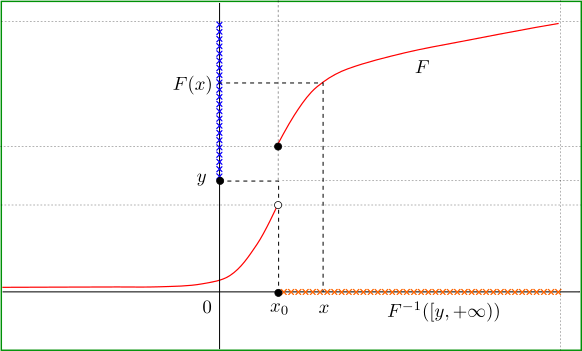
\includegraphics[width=0.8\textwidth]{Figuras/inversa-gen.pdf}
\caption{Gráfico de uma função distribuição descontínua.}
\label{Rotulo}
\end{figure}
\end{center}
%%%
\end{observacao}

\begin{proposicao}\label{prop-propriedades-G}
	Para todo $y\in (0,1)$ o conjunto $A(y)$ definido acima 
	tem as seguintes propriedades:
	\begin{enumerate}
		\item 
		$A(y)$ é um conjunto fechado.
		
		\item
		$\inf A(y) \in A(y)$, ou seja, $y\leq F(G(y))$.
		
		\item 
		$t<G(y)$ se, e somente se, $F(t)<y$.
		
		\item 
		$G(y)\leq t$ se, e somente se, $y\leq F(t)$.
	\end{enumerate}
\end{proposicao}


\begin{proof}
	{\bf Prova do item 1.} 
	Seja $\{s_n\}$ uma sequência em $A(y)$ tal que $s_n\to s$. 
	Note que $\{s_n\}$ possui pelo menos uma subsequência 
	monótona, não-crescente ou não-decrescente $\{s_{n_{k}}\}$ 
	que converge para $s$. Vamos considerar primeiro o caso 
	em que existe uma subsequência $s_{n_k}\downarrow s$. 
	Já que $s_{n_k}\in A(y)$ então 
	é válida a seguinte desigualdade $y\leq F(s_{n_k})$.
	Tomando o limite, quando $k\to\infty$, nesta desigualdade 
	obtemos da continuidade a direita de $F$ que 
		\[ 
			y \leq 
			\lim_{k\to\infty} F(s_{n_k}) 
			= 
			F(s).
		\]
	O que mostra que $s\in A(y)$.
	Por outro lado, se $\{s_n\}$ não possui uma subsequência 
	$s_{n_k}\downarrow s$, então existe no máximo uma quantidade
	finita de pontos da sequência $\{s_n\}$ 
	que é maior ou igual a $s$.
	Assim podemos afirmar que existe pelo menos 
	uma subsequência $s_{n_k}\uparrow s$
	tal que $s_{n_k} < s$. Usando  
	a definição de $A(y)$ e a monotonicidade de $F$ 
	temos que 
		\[
			y\leq F(s_{n_k})\leq F(s).
		\]
	Logo $s\in A(y)$ e isto conclui a prova de que $A(y)$ é 
	um subconjunto fechado da reta.
	
	{\bf Prova do item 2.} Segue diretamente da definição $\inf A(y)$,
	que 	existe uma sequência $\{s_n\}\subset A(y)$ tal que $s_n\to \inf A(y)$.
	Uma vez que o item 1 garante que $A(y)$ é fechado, temos que 
		\[G(y)=\inf A(y) \in A(y).\]
	 Segue então da definição de $A(y)$ que $y\leq F(G(y))$.


	{\bf Prova do item 3.} Note que $t<G(y)$ é equivalente a
	$t<\inf A(y)$. Esta desigualdade é equivalente a 
	$t\in A(y)^c$, isto é, $t\in\{s\in\R: F(s)<y\}$. 
	Como a última afirmação é equivalente a $F(t)<y$ a
	prova deste item está completa.
	
	
	{\bf Prova do item 4.} Se $G(y)\leq t$ então 
	segue do item 3 que 	$y\leq F(t)$. A recíproca é 
	também uma aplicação direta do item 3.  
	Isto completa a prova da proposição.
\end{proof}

\bigskip

Para cada $A\subset \R$ definimos agora o seguinte conjunto:
	\begin{equation}\label{def-xi-F}
		\xi_F(A) \equiv \{ x\in (0,1]: G(x)\in A \} = G^{-1}(A)\cap (0,1].
	\end{equation}
No lema seguinte mostramos que se $A$ 
é um boreliano de $\R$ (notação $A\in\mathscr{B}(\R)$)  
então 
$\xi_F(A)$ é um boreliano de $(0,1]$ 
(notação $\xi_F(A) \in\mathscr{B}((0,1])$).

\begin{lema}
	Se $A\in\mathscr{B}(\R)$ então $\xi_F(A) \in\mathscr{B}((0,1])$, onde
	$\xi_F(A)$ é dada em \eqref{def-xi-F}.
\end{lema}



\begin{proof}
Considere a seguinte coleção 
	\[
		\mathscr{C} 
		=
		\{ A\subset\R: \xi_F(A) \in \mathscr{B}((0,1])\}.
	\]
Afirmamos que $\mathscr{C}$ contém qualquer intervalo finito da forma
$(a,b]\subset \R$. De fato, segue dos item 3 e 4 
da Proposição \ref{prop-propriedades-G} que 
para todo $x\in (0,1)$ satisfazendo 
$a<G(x)$ temos $F(a)<x$ e se $G(x)\leq b$ então 
$x\leq F(b)$. Da definição de $\xi_{F}(A)$ e 
das duas observações anteriores temos que
%
%
\begin{align*}
	\xi_F(A) 
	&= 
	\{ x\in (0,1]: G(x) \in (a,b] \}
	\\
	&=	
	\{ x\in (0,1]: a<G(x)\leq b  \}
	\\
	&=
	\{ x\in (0,1]:F(a) <x \leq F(b) \}
	\\
	&=
	(F(a),F(b)].
\end{align*}
Como o lado direito da igualdade pertence a $\mathscr{B}((0,1])$
segue que todo intervalo finito $(a,b]\in \mathscr{C}$.
Em outras palavras, a coleção $\mathscr{C}$ 
contém o $\pi$-sistema $\mathcal{G}=\{ (a,b]: a,b\in\R\}$.


Vamos mostrar agora que $\mathscr{C}$ é um $\lambda$-sistema. 
Para provar que $\R\in \mathscr{C}$, basta 
notar que
$
	\xi_F(\R)
	= G^{-1}(\mathbb{R})\cap (0,1] 
	= (0,1)\cap (0,1]
	\in \mathscr{B}((0,1]). 
$
Suponha que $A\in\mathscr{C}$, então 
$\xi_F(A)=G^{-1}(A)\cap (0,1]\in \mathscr{B}((0,1])$.
Pela propriedades de imagem inversa temos que 
\[
	G^{-1}(A^c)= \Big(G^{-1}(A)\Big)^c
\]
e como $\xi_F(A)$ é um boreliano de $(0,1]$, segue da definição 
de topologia induzida que 
	\[
		\xi_F(A^c)
		=
		G^{-1}(A^c)\cap (0,1]
		= 
		\Big(G^{-1}(A)\Big)^c\cap (0,1]		
	\]
é um boreliano de $(0,1]$, mostrando que $A^c\in\mathscr{C}$.

Se $\{A_n\}$ é uma família de 
conjuntos mutuamente disjuntos em $\mathscr{C}$,
então 
	\begin{align*}
	\xi_F\left( \bigcup_{n=1}^{\infty} A_n\right)
	=&
	G^{-1}\left( \bigcup_{n=1}^{\infty} A_n\right)\cap (0,1]
	\\
	=&
	\bigcup_{n=1}^{\infty} G^{-1}\left(A_n \right)\cap (0,1]
	\end{align*}
pertence a $\mathscr{B}((0,1])$. Logo $\cup_{n\geq 1} A_n\in \mathscr{C}$
o que prova encerra a prova de que $\mathscr{C}$ é um $\lambda$-sistema.

Pelo Teorema $\pi-\lambda$ de Dynkin $\mathscr{C}$ contém a $\sigma$-álgebra
gerada por $\mathcal{G}$ que é $\mathscr{B}(\R)$. Este fato 
completa a prova do lema.
\end{proof}

Finalmente podemos apresentar a definição de $\P_F$.
Para cada $A\in \mathscr{B}(\R)$ definimos 
	\[
		\P_{F}(A) =\lambda(\xi_{F}(A)),
	\]
onde $\lambda$ é a medida de Lebesgue em $(0,1]$.
É simples verificar que $\P_F$ é de fato uma medida
de probabilidade e que sua distribuição é dada por
%
\begin{align*}
	\P_F((-\infty,x]) 
	&=
	\lambda \Big(\xi_{F}((-\infty,x])\Big)
	\\
	&=
	\lambda\Big( \{ y\in (0,1]: G(y)\in (-\infty,x] \} \Big)
	\\
	&=
	\lambda\Big( \{ y\in (0,1]: G(y)\leq x \} \Big)
	\\
	&=
	\lambda\Big( \{ y\in (0,1]: y\leq F(x) \} \Big)
	\qquad
	(\text{item 4 Proposição \ref{prop-propriedades-G}})
	\\
	&=
	\lambda\Big( (0,F(x)] \Big)
	\\
	&=
	F(x).
\end{align*}
















% Aula 5
\chapter[Aula 5]{Funções Mensuráveis e Variáveis Aleatórias}
\chaptermark{}

\section{Funções Mensuráveis}

Denotamos por $\overline{\R}$ a reta estendida, isto é, 
$\overline{\R} = \R\cup\{-\infty,+\infty\}$. Podemos 
estender naturalmente conceito de soma e produto 
para os seguintes pares de elementos 
de $\overline{\R}$ da seguinte maneira:
\begin{enumerate}
	\item 
	Se $x,y\in \R$ a soma é a soma usual 
	e o mesmo para o produto. 
	
	\item para todo $x\in \overline{R}$ temos 
	$0\cdot x=0$.
	
	\item Para todo $x\in \overline{R}$ diferente de 
	$-\infty$ definimos $x+(+\infty)=+\infty$.

	\item Para todo $x\in \overline{R}$ diferente de 
	$+\infty$ definimos $x+(-\infty)=-\infty$.
\end{enumerate}

Não vamos nos preocupar neste momento em munir $\overline{\R}$ 
de uma topologia, mas vamos definir a $\sigma$-álgebra
de Borel de $\overline{R}$,
como sendo a coleção formada pela reunião da
coleção $\mathscr{B}(\R)$ 
e de todos conjuntos da forma 
$B\cup\{-\infty\}$, $B\cup\{+\infty\}$ e $B\cup\{-\infty,+\infty\}$,
onde $B$ varia sobre todos os elementos de $\mathscr{B}(\R)$.
Esta coleção que acabamos de definir
é de fato uma $\sigma$-álgebra e será chamada de $\sigma$-álgebra
de borel de $\overline{R}$ e denotada por $\mathscr{B}(\overline{\R})$.

\begin{exercicio}
	Mostre que a coleção $\mathscr{B}(\overline{\R})$ 
	é uma $\sigma$-álgebra.
\end{exercicio}

\begin{exercicio}
	Podemos ver $\overline{R}$ como um conjunto totalmente ordenado se 
	consideramos a relação de ordem ``$<$'' obtida pela extensão natural 
	da relação de ordem em $\R$.
	Seja $\tau$ a topologia da ordem definida por ``$<$'' 
	em $\overline{R}$. Mostre que a $\sigma$-álgebra gerada pelos 
	abertos de $\tau$ coincide com a coleção $\mathscr{B}(\overline{\R})$
	definida acima. 
	
\end{exercicio}










\subsection*{Funções a Valores Reais Mensuráveis}

Nesta subseção vamos considerar funções que
saem de um espaço mensurável $(\Omega,\F)$ e toma 
valores em $\mathbb{R}$. O caso mais geral, onde
as funções assumem valores em $\overline{R}$ será
tratado na subseção seguinte.


\begin{definicao} 
Seja $(\Omega,\F)$ um espaço mensurável. 
Uma função $f:\Omega\to\R$ é dita $\F$-mensurável
se para todo número real $\alpha$ temos que
\[
	\{x\in\Omega : f(x)>\alpha \} \in \F.
\]
\end{definicao}

O próximo lema fornece três maneira alternativas de
definir funções mensuráveis. 

\begin{lema}
As seguintes afirmações são equivalentes para uma função 
$f:\Omega\to\R$.
\begin{enumerate}
	\item 
	Para todo $\alpha\in\R$ o conjunto 
	$A_{\alpha}\equiv\{x\in\Omega : f(x)>\alpha \} \in \F$.

	\item 
	Para todo $\alpha\in\R$ o conjunto 
	$B_{\alpha}\equiv\{x\in\Omega : f(x)\leq \alpha \} \in \F$.

	\item 
	Para todo $\alpha\in\R$ o conjunto 
	$C_{\alpha}\equiv\{x\in\Omega : f(x)\geq\alpha \} \in \F$.

	\item 
	Para todo $\alpha\in\R$ o conjunto 
	$D_{\alpha}\equiv\{x\in\Omega : f(x)<\alpha \} \in \F$.
	
\end{enumerate}
\end{lema}



% Lista 1
\chapter*{Lista 1}
\addcontentsline{toc}{chapter}{Lista 1}
\chaptermark{}
%%%%%%%%%%%%%%%%%%%%%%%%%%%%%%%%%%%%%%%%%%%%%%%%

% Inicio da Lista de Exercícios 
\begin{enumerate}[leftmargin=*]

\item 
Exercício 1.


\item 
Exercício 2.


\end{enumerate}
%  Fim da Lista de Exercícios





% Aula 6
\chapter[Aula 6]{Variáveis Aleatórias e Independência}
\chaptermark{}

\section{Variáveis Aleatórias}

\begin{definicao}[Variável Aleatória]\label{def-var-aleatoria}
Seja $(\Omega,\F)$ um espaço de medida e $\Lambda\in\F$.
Uma função $X:\Lambda\to\overline{\R}$ tal que para todo 
$B\in\mathscr{B}(\overline{\R})$ temos 
	\[
		\{\omega \in\Lambda: X(\omega)\in B\} 
		\in \Lambda\cap\F,
	\]
onde $\Lambda\cap \F$ denota a coleção de todos os 
subconjuntos de $\Omega$ da forma $\Lambda\cap F$
com $F\in\F$.
\end{definicao}

\begin{observacao}
Esta definição nesta generalidade é necessária por razões
lógicas em algumas aplicações, mas para a discussão das
propriedades básicas de variáveis aleatórias, podemos 
supor que $\Lambda =\Omega$.
\end{observacao}


\begin{exercicio}
Suponha que $\Lambda=\Omega$ na Definição \ref{def-var-aleatoria}.
Mostre que uma variável aleatória é uma função $\F$-mensurável
tomando valores em $\overline{\R}$ no sentido da seção anterior.  
\end{exercicio}








%%%%%%%%%%%%%%%%%% Referências e Índice Remissivo
\backmatter
%
%\chapter{Referências}
%\include{./referencias/referencias}

\printindex
%\chapter{Índice de Símbolos}


\end{document}
